\documentclass[conference]{IEEEtran}
\IEEEoverridecommandlockouts

\usepackage{cite}
\usepackage{amsmath,amssymb,amsfonts}
\usepackage{graphicx}
\usepackage{textcomp}
\usepackage{xcolor}
\usepackage{booktabs}
\usepackage{array}
\usepackage{multirow}
\usepackage{tikz}
\usetikzlibrary{shapes.geometric,arrows.meta,positioning,fit,backgrounds,calc}
\usepackage{pgfplots}
\pgfplotsset{compat=1.17}
\usepackage{url}
\usepackage{flushend}   % balance the two columns on the final page
\usepackage[hidelinks]{hyperref}

\def\BibTeX{{\rm B\kern-.05em{\sc i\kern-.025em b}\kern-.08em
    T\kern-.1667em\lower.7ex\hbox{E}\kern-.125emX}}

% Compact spacing to fit an extended report while keeping IEEE style
\setlength{\parskip}{2pt}

\begin{document}

\title{Cloud-Native Construction Project Intelligence Platform for Predictive Delay-Risk Scoring and Real-Time Performance Analytics}

\author{
\IEEEauthorblockN{Hasnain Makada\textsuperscript{1}, Sahil Mall\textsuperscript{1}, Aryan Kishor Sao\textsuperscript{1}}
\IEEEauthorblockA{\textsuperscript{1}School of Computer Science and Engineering,\\
Vellore Institute of Technology, Vellore, India\\
\{hasnain.makada, sahil.mall, aryan.kishorsao\}@vitstudent.ac.in}
\and
\IEEEauthorblockN{Dr. Manikandan K}
\IEEEauthorblockA{Professor Grade 2,\\
Department of Database Systems,\\
School of Computer Science and Engineering,\\
Vellore Institute of Technology, Vellore, India\\
kmanikandan@vit.ac.in}
}

\maketitle

\begin{abstract}
Construction project controls depend on tracking the triple constraints of schedule, cost, and scope, yet contemporary management workflows remain hindered by fragmented reporting mechanisms, retrospective performance indices, and a systemic separation between analytical computation and software deployment infrastructure. Existing studies frequently investigate visual dashboards, schedule-delay models, or cloud storage in isolation, leaving a critical gap in deployable, reproducible systems. This paper presents the architecture, implementation, and empirical evaluation of a cloud-native construction project intelligence platform that integrates project-control data across containerized microservices and automated visual analytics. The system comprises five integrated layers: (i) a standardized data-ingestion pipeline implemented in Python and FastAPI that validates every record against strict schemas; (ii) a relational PostgreSQL database structuring master project parameters and append-only time-series progress updates; (iii) an analytics engine executing Earned Value Management and probabilistic delay-risk forecasting through supervised machine-learning classification and a differentiable reliability formulation; (iv) a decision-support layer realized through an interactive web dashboard and Microsoft Power BI; and (v) a reproducible cloud-native orchestration topology deployed on Kubernetes using Docker containers. We demonstrate how the platform unifies retrospective variance metrics with predictive risk scoring, enabling continuous schedule-cost visibility and early delay detection. On a reproducible activity-level dataset of six projects and 300 activities, the calibrated Gradient Boosting classifier achieved a ROC-AUC of 0.976 and the system sustained end-to-end ingestion of 19,017 records with zero validation rejections. All Earned Value identities were verified across 189 computed KPI rows, and Kubernetes failover recovered a terminated ingestion pod within approximately one second. The platform thereby translates the fragmented promises of prior work into a single, open, and reproducible operating system for project control.
\end{abstract}

\begin{IEEEkeywords}
construction project intelligence, Earned Value Management, delay-risk prediction, machine learning, Power BI, Docker, Kubernetes, cloud-native architecture, visual analytics.
\end{IEEEkeywords}

% ============================================================================
\section{Introduction}
% ============================================================================

Civil engineering and capital construction projects are characterized by high operational complexity, multifaceted trade interdependencies, and strict contractual schedules. Despite significant advancements in digital scheduling platforms such as Oracle Primavera P6 and Microsoft Project, cost overruns and schedule slippage remain endemic across the global construction industry. A substantial root cause of project distress is delayed visibility: progress and financial records are traditionally collected through manual site logs, disparate spreadsheets, and disconnected subcontractor reports. Consequently, schedule and cost variances are identified only after periodic commercial meetings---long after corrective interventions could have prevented budget and timeline damage.

Industry 4.0 initiatives have introduced automated data acquisition mechanisms, including Building Information Modeling (BIM), Quick Response (QR) field scanning, and Internet of Things (IoT) sensors. Furthermore, Business Intelligence (BI) platforms---predominantly Microsoft Power BI---have demonstrated efficacy in synthesizing complex project data into interactive dashboards. However, current industry practice exhibits three severe systemic deficiencies.

\textbf{(1) Data Fragmentation and Processing Latency.} Site records, cost sheets, and baseline schedules reside in siloed applications without a unified schema, forcing project teams to manually reconstruct reporting models at every reporting cycle. The absence of a normalized, auditable data substrate means that each analytical exercise begins from an inconsistent foundation.

\textbf{(2) Retrospective Metrics Rather Than Predictive Insight.} Standard project monitoring relies on deterministic Earned Value Management (EVM) formulas. While indices such as the Cost Performance Index (CPI) and the Schedule Performance Index (SPI) describe historical performance, they lack probabilistic forecasting mechanisms to warn project managers of future activity-level delay vulnerabilities before critical-path activities slip.

\textbf{(3) Disconnection Between Analytical Models and Production Deployment.} Advanced predictive algorithms and delay-risk reliability models published in the civil engineering literature are typically implemented as isolated research scripts. They lack reproducible, containerized software architectures capable of auto-scaling, managing secrets, and sustaining continuous integration within enterprise IT ecosystems.

To address these limitations, this paper proposes and empirically evaluates an end-to-end, reproducible, cloud-native construction project intelligence platform. The platform couples containerized Python data pipelines with PostgreSQL storage, integrates machine learning and probabilistic delay-risk modeling, and exposes decision-ready semantic views directly to interactive web and Power BI dashboards, all orchestrated across a resilient Kubernetes cluster.

The principal contributions of this work are as follows:
\begin{itemize}
  \item \textbf{A unified architecture} that composes ingestion, persistence, analytics, prediction, and presentation into a single decoupled, microservice-based system, closing the integration gap identified across prior studies.
  \item \textbf{A three-tier normalized data model} that separates master entities, append-only time-series facts, and computed analytical outputs, enabling auditable lineage from raw field data to decision dashboards.
  \item \textbf{An automated EVM engine} that computes the full indicator set (CV, SV, CPI, SPI, EAC, TEAC) at a per-project status date, with a validation protocol that verifies every algebraic identity against stored results.
  \item \textbf{A predictive delay-risk engine} that frames schedule slippage as supervised binary classification and augments it with a differentiable softmax surrogate of the Critical Path Method (CPM) max operator to estimate the most probable point of schedule failure.
  \item \textbf{A reproducible cloud-native deployment} packaged with Docker and orchestrated on Kubernetes, featuring health probes, horizontal pod autoscaling, persistent storage, and a verified self-healing failover characteristic.
  \item \textbf{A fully open, one-command reproducibility protocol} across Linux, macOS, and Windows, accompanied by a synthetic activity-level dataset generator that supplies the baselines and delay labels necessary for genuine EVM and valid classification.
\end{itemize}

\subsection{Background and Motivation}

Digital transformation in construction informatics has historically advanced along three loosely coupled fronts: field data capture, analytical modeling, and management reporting. Data-capture technologies such as BIM authoring tools, QR-based field scanning, and IoT sensing have matured rapidly. Analytical modeling---ranging from deterministic Earned Value formulations to probabilistic schedule-reliability methods and machine-learning classifiers---has likewise advanced. Management reporting, meanwhile, has converged on interactive business-intelligence platforms, with Microsoft Power BI emerging as a de facto standard in project-control practice. The connective tissue between these fronts, however, has not kept pace. In the absence of a unifying architecture, the integration effort is repeatedly deferred to manual reporting, where data is reconciled across spreadsheets at each reporting cycle.

This deferral has measurable operational consequences. Because reconciliation is manual, reporting latency grows with project size and with the number of participating subcontractors. Because the resulting models are rebuilt from scratch each cycle, lineage is lost and errors are difficult to attribute. Because analytics and reporting evolve independently, a predictive model validated in one environment may not be reproducible in another. The cumulative effect is a project-control workflow that is accurate in retrospect but blind in prospect.

\subsection{Problem Statement}

Let a portfolio consist of projects $P = \{p_1, \dots, p_n\}$, each composed of activities $A_{p}$, each activity carrying a planned budget, baseline dates, and a stream of append-only progress and cost observations. Let $\mathcal{S}$ denote the schema imposed on these observations and $\mathcal{C}$ the set of validation constraints that a well-formed record must satisfy. The project-control problem addressed here is to construct a mapping
\begin{equation}
\Phi : (\mathcal{P}, \mathcal{O}) \longmapsto (\mathcal{K}, \mathcal{R})
\end{equation}
from the project definitions $\mathcal{P}$ and the observation streams $\mathcal{O}$ to a set of Earned Value indicators $\mathcal{K}$ and predictive risk scores $\mathcal{R}$, such that (i) every admitted observation satisfies $\mathcal{C}$, (ii) every indicator in $\mathcal{K}$ satisfies its defining algebraic identity, and (iii) the mapping is reproducible---that is, a function only of the inputs and a fixed random seed, independent of the execution environment.

Existing practice fails these conditions in characteristic ways: constraint (i) is unenforced where ingestion is manual; constraint (ii) is unverified where indicators are computed ad hoc; and constraint (iii) is unmet where analyses exist as notebooks rather than versioned services. The platform is engineered so that all three conditions hold simultaneously.

\subsection{Research Questions}

The evaluation is organized around four research questions:
\begin{itemize}
  \item \textbf{RQ1 (Integrity).} Can heterogeneous project records be ingested through a strict validation gate without loss of well-formed data?
  \item \textbf{RQ2 (Analytical correctness).} Can the full Earned Value indicator set be computed automatically such that every algebraic identity holds across all stored results?
  \item \textbf{RQ3 (Predictive quality).} How well do candidate classifiers distinguish delayed from on-time activities, and which model best balances discrimination and alerting utility?
  \item \textbf{RQ4 (Deployment resilience).} Does the containerized deployment exhibit self-healing and autoscaling behavior suitable for continuous operation?
\end{itemize}

The remainder of this paper is organized as follows. Section~II presents the system model and architecture. Section~III reviews the literature and related work. Section~IV analyzes existing approaches and their limitations. Section~V details the proposed design. Section~VI describes the implementation. Section~VII presents the result analysis, including threats to validity. Sections~VIII and~IX conclude and outline future work, respectively.

% ============================================================================
\section{System Model and Architecture}
% ============================================================================

\subsection{Design Philosophy}

The platform is structured as a cloud-native, microservices-driven intelligence system. Its architecture deliberately decouples data ingestion, persistence, heavy analytics, and front-end visualization, ensuring that failures in dashboard refreshes or analytical scaling do not compromise data-capture integrity. This separation of concerns follows directly from the observation that construction data capture must remain available even when analytical or presentation tiers are degraded.

The high-level data flow is:
\begin{center}
\emph{Project Data $\rightarrow$ Ingestion API $\rightarrow$ PostgreSQL $\rightarrow$ Analytics + Delay-Risk Service $\rightarrow$ Curated Views $\rightarrow$ Web UI / Power BI}
\end{center}

\subsection{Overall System Topology}

Raw project data flows from external sources through an ingress layer into containerized FastAPI ingestion pods. Normalized records are stored in a persistent PostgreSQL cluster, after which independent analytics and risk pods execute EVM and predictive algorithms, writing outputs back to dedicated database tables for downstream consumption by the web dashboard and Power BI. Figure~\ref{fig:arch} illustrates the end-to-end topology.

\begin{figure}[t]
\centering
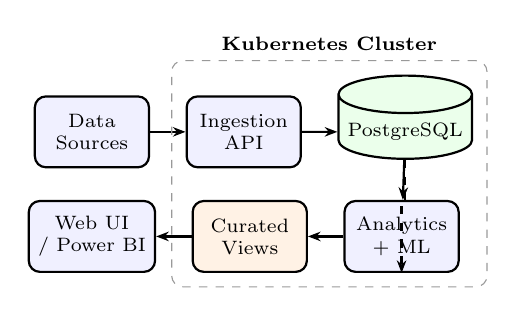
\begin{tikzpicture}[
  node distance=0.4cm and 0.45cm,
  box/.style={rectangle, rounded corners, draw=black, thick, fill=blue!6, minimum width=1.45cm, minimum height=0.9cm, align=center, font=\scriptsize},
  db/.style={cylinder, shape border rotate=90, aspect=0.28, draw=black, thick, fill=green!8, minimum width=1.3cm, minimum height=1.05cm, align=center, font=\scriptsize},
  outbox/.style={rectangle, rounded corners, draw=black, thick, fill=orange!10, minimum width=1.45cm, minimum height=0.9cm, align=center, font=\scriptsize},
  arr/.style={-{Stealth[length=1.6mm]}, thick}
]
\node[box] (src) {Data\\Sources};
\node[box, right=of src] (ing) {Ingestion\\API};
\node[db, right=of ing] (pg) {PostgreSQL};
\node[box, below=of src] (ui) {Web UI\\/ Power BI};
\node[outbox, right=of ui] (cv) {Curated\\Views};
\node[box, right=of cv] (ana) {Analytics\\+ ML};
\draw[arr] (src) -- (ing);
\draw[arr] (ing) -- (pg);
\draw[arr] (pg) -- (ana);
\draw[arr] (ana) -- (cv);
\draw[arr] (cv) -- (ui);
\draw[arr, dashed] (pg.south) -- ++(0,-0.55) -| (ana.south);
\node[draw=black!40, dashed, rounded corners, fit=(ing)(pg)(ana)(cv), inner sep=5pt, label={[font=\scriptsize\bfseries]above:Kubernetes Cluster}] (clus) {};
\end{tikzpicture}
\caption{End-to-end system topology. Kubernetes orchestrates every backend service with health probes, autoscaling, and persistent storage.}
\label{fig:arch}
\end{figure}

\subsection{The Unified Data Model}

To eliminate reporting silos, the platform employs a relational schema organized into three functional tiers: master entities, time-series fact records, and computed output tables. This three-tier separation mirrors the conceptual distinction between stable project definitions, evolving field observations, and derived analytical results.

\textbf{Master Data.} The \texttt{Project} and \texttt{Activity} entities define baseline schedule boundaries, planned start and finish dates, and planned resource budgets. These records change infrequently and represent the contractual and planning reference against which performance is measured.

\textbf{Time-Series Fact Records.} The \texttt{ProgressUpdate}, \texttt{CostRecord}, and \texttt{ResourceRecord} entities store append-only logs of field execution. Progress updates track actual physical percentages and the corresponding earned value; cost records accumulate the actual cost (AC) incurred; resource records capture labor, equipment, and material consumption.

\textbf{Computed Output Tables.} The \texttt{KPIResult} and \texttt{RiskResult} entities store calculated Earned Value metrics and machine-learning delay probabilities generated by the backend analytical services. Because these are recomputable, they are isolated from the source facts, allowing analytical recalibration without mutating raw observations.

Table~\ref{tab:entities} summarizes the principal entities and their key attributes.

\begin{table}[t]
\caption{Principal Entities of the Three-Tier Data Model}
\label{tab:entities}
\centering
\footnotesize
\begin{tabular}{@{}p{1.35cm}p{0.85cm}p{4.4cm}@{}}
\toprule
\textbf{Entity} & \textbf{Tier} & \textbf{Key Attributes} \\
\midrule
Project & Master & project\_id, name, contractor, budget\_at\_completion, planned dates \\
Activity & Master & activity\_id, WBS, trade, planned dates, budget, float, criticality, predecessor count \\
ProgressUpdate & Fact & activity, timestamp, percent\_complete, planned\_value (PV), earned\_value (EV) \\
CostRecord & Fact & activity, timestamp, actual\_cost (AC) \\
ResourceRecord & Fact & activity, timestamp, workers, equipment utilization, material usage \\
KPIResult & Output & PV, EV, AC, CV, SV, CPI, SPI, EAC, TEAC \\
RiskResult & Output & delay probability, risk category, model version, top features \\
\bottomrule
\end{tabular}
\end{table}

\subsection{Formal Data Model}

We formalize the schema so that the later correctness claims can be stated precisely. A \emph{project} is a tuple
\begin{equation}
p = \langle \mathit{id}, \mathit{bac}, s_0, f_0 \rangle
\end{equation}
where $\mathit{bac} \in \mathbb{R}^+$ is the budget at completion and $s_0, f_0$ are planned start and finish dates with $s_0 \le f_0$. An \emph{activity} extends this with
\begin{equation}
a = \langle \mathit{id}, p, d, b, \phi, k, \rho \rangle
\end{equation}
where $d$ is the planned duration in days, $b$ the activity budget, $\phi \ge 0$ the total float, $k \in \{0,1\}$ a criticality flag, and $\rho \in [0,1]$ a historical subcontractor delay rate.

A \emph{progress observation} at time $t$ for activity $a$ is $u = \langle a, t, \pi, v, w \rangle$ with $\pi \in [0,100]$ the percent complete, $v \ge 0$ the earned value, and $w \ge 0$ the planned value at $t$. Because observations are append-only, the sequence $\{u_{a,t}\}$ for a fixed activity is totally ordered by $t$, and the \emph{status value} at a status date $T$ is the observation with maximal $t \le T$. A \emph{cost observation} is $c = \langle a, t, \kappa \rangle$ with $\kappa \in \mathbb{R}$ the incremental actual cost.

The \emph{computed} tier consists of KPI rows
\begin{equation}
\kappa_a = \big\langle \mathrm{PV}, \mathrm{EV}, \mathrm{AC}, \mathrm{CV}, \mathrm{SV}, \mathrm{CPI}, \mathrm{SPI}, \mathrm{EAC}, \mathrm{TEAC} \big\rangle
\end{equation}
and risk rows $r_a = \langle \hat{y}_a, \ell_a, \mu \rangle$ with $\hat{y}_a \in [0,1]$ a predicted delay probability, $\ell_a \in \{\text{Low},\text{Medium},\text{High}\}$ a category, and $\mu$ a model version. Because the computed tier is derivable from the fact tier and the master tier, it can be regenerated at will, which is the property that supports analytical recalibration without mutation of raw observations.

A key invariant concerns the \emph{status date}. Define the cumulative actual cost to date $T$ as
\begin{equation}
\mathrm{AC}(a,T) = \sum_{t \le T} \kappa_{a,t},
\end{equation}
and let $(\mathrm{PV}_{a,T}, \mathrm{EV}_{a,T})$ be the planned and earned value of the status observation at or before $T$. The indicators are then computed exactly as in Table~\ref{tab:evm}. The status date $T_p$ for project $p$ is chosen as the midpoint of that project's reporting window,
\begin{equation}
T_p = \tfrac{1}{2}\big(\min_{a \in A_p} t_{\min}(a) + \max_{a \in A_p} t_{\max}(a)\big),
\end{equation}
which guarantees a mid-execution snapshot for every project in a staggered portfolio.

\subsection{Data Dictionary}

Table~\ref{tab:dict} specifies the physical attributes of the principal relations, including their domains and validation constraints. The constraints are enforced at the ingestion boundary and mirrored at the schema level where possible.

\begin{table}[t]
\caption{Data Dictionary of Principal Relations}
\label{tab:dict}
\centering
\scriptsize
\setlength{\tabcolsep}{2.5pt}
\begin{tabular}{@{}p{1.4cm}p{1.9cm}p{1.3cm}p{1.15cm}@{}}
\toprule
\textbf{Relation} & \textbf{Attribute} & \textbf{Domain} & \textbf{Rule} \\
\midrule
Project & project\_id & string & PK \\
Project & budget\_at\_completion & real & $>0$ \\
Project & planned\_start, \_finish & date & start$\le$finish \\
Activity & activity\_id & string & PK \\
Activity & project\_id & string & FK \\
Activity & planned\_duration & real & $\ge 0$ \\
Activity & budget & real & $>0$ \\
Activity & total\_float & real & $\ge 0$ \\
Activity & is\_critical & bool & $\{0,1\}$ \\
Activity & sub\_delay\_rate & real & $[0,1]$ \\
Progress & timestamp & tstz & tz-aware \\
Progress & percent\_complete & real & $[0,100]$ \\
Progress & earned/planned\_val & real & $\ge 0$ \\
CostRecord & actual\_cost & real & signed \\
Resource & worker\_count & int & $\ge 0$ \\
Resource & equip\_utilization & real & $[0,100]$ \\
\bottomrule
\end{tabular}
\end{table}

\subsection{Entity-Relationship Structure}

Figure~\ref{fig:er} depicts the entity-relationship structure of the schema. A project aggregates many activities; each activity owns many progress, cost, and resource observations; and each activity resolves to at most one current KPI row and one current risk row through the curated views. The cardinalities are one-to-many from project to activity and from activity to each fact relation, and one-to-one (at the latest snapshot) from activity to each computed relation.

\begin{figure}[t]
\centering
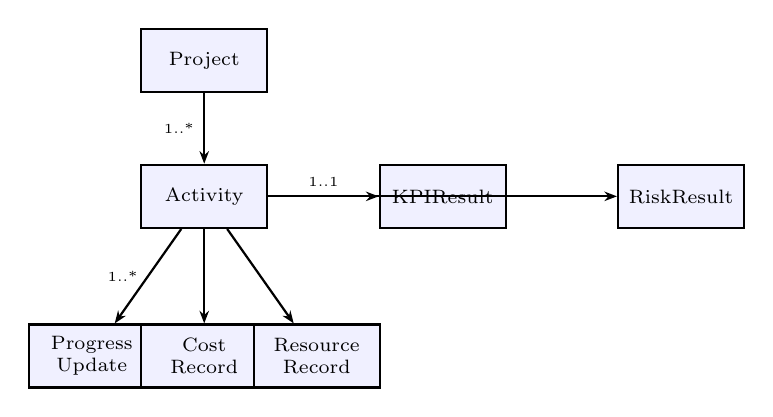
\begin{tikzpicture}[
  ent/.style={rectangle, draw=black, thick, fill=blue!6, minimum width=1.6cm, minimum height=0.8cm, align=center, font=\scriptsize},
  arr/.style={-{Stealth[length=1.6mm]}, thick}
]
\node[ent] (proj) {Project};
\node[ent, below=0.9cm of proj] (act) {Activity};
\node[ent, below left=1.2cm and -0.2cm of act] (prg) {Progress\\Update};
\node[ent, below=1.2cm of act] (cost) {Cost\\Record};
\node[ent, below right=1.2cm and -0.2cm of act] (res) {Resource\\Record};
\node[ent, right=1.4cm of act] (kpi) {KPIResult};
\node[ent, right=1.4cm of kpi] (risk) {RiskResult};
\draw[arr] (proj) -- node[left,font=\tiny]{1..*} (act);
\draw[arr] (act) -- node[left,font=\tiny]{1..*} (prg);
\draw[arr] (act) -- (cost);
\draw[arr] (act) -- (res);
\draw[arr] (act) -- node[above,font=\tiny]{1..1} (kpi);
\draw[arr] (act) -- (risk);
\end{tikzpicture}
\caption{Entity-relationship structure: master entities aggregate fact observations and resolve to computed outputs.}
\label{fig:er}
\end{figure}

\subsection{Containerized Microservices and Deployment Topology}

\textbf{Ingestion Service (FastAPI).} Implemented in Python, this service provides high-speed asynchronous REST endpoints that validate inbound JSON payloads against strict Pydantic schemas, rejecting malformed data with standard HTTP 422 error codes. Validation occurs before any persistence, guaranteeing that invalid records never reach the analytical tier.

\textbf{Database Storage (PostgreSQL).} Deployed within Kubernetes as a StatefulSet attached to persistent disk volumes, PostgreSQL maintains ACID compliance and preserves historical data across container recreation.

\textbf{Analytics and Delay-Risk Services.} Stateless worker pods running Pandas, NumPy, and Scikit-learn execute scheduled batch jobs for variance computation and probabilistic delay classification.

\textbf{Orchestration Layer (Kubernetes).} The platform automates deployment scaling via Horizontal Pod Autoscaling (HPA), isolates credentials using Kubernetes Secrets, and executes liveness and readiness probes to self-heal failed microservices.

% ============================================================================
\section{Literature Review and Related Works}
% ============================================================================

The following review organizes prior research across four threads that together motivate the present platform: construction data visualization and business intelligence, delay prediction and probabilistic risk modeling, cloud-based and cloud-native data management, and data-driven decision-making.

\subsection{Construction Project Visualization and Business Intelligence}

Visual analytics provides project stakeholders with intuitive, multi-dimensional representations of progress data. Chiu and Russell~\cite{chiu2011design} pioneered the structured development of construction data visualization environments, demonstrating that top-down visual frameworks improve schedule comprehension and task-status identification compared with static Gantt charts. However, their early framework remained schedule-centric, lacking dynamic linkages to cost control, resource consumption, or automated prediction.

With the maturation of enterprise analytics, business-intelligence dashboards have gained widespread traction. Al-Sulaiti \emph{et al.}~\cite{alsulaiti2021using} developed Power BI dashboards to consolidate Engineering, Procurement, and Construction (EPC) key performance indicators, validating that dynamic reporting elevates management visibility and enhances multi-stakeholder collaboration. In a survey across construction practitioners, Ghosh \emph{et al.}~\cite{ghosh2024use} reported that a large share of industry professionals utilize Power BI as their primary visualization platform, while the absence of real-time data integration and the prevalence of inaccurate or incomplete project data constitute the greatest barriers to dashboard effectiveness.

Abdulaziz and Ahmed~\cite{abdulaziz2026customized} established a customized Power BI dashboard integrated with BIM for residential structures, demonstrating how Data Analysis Expressions (DAX) measures automate the computation of cumulative planned value, earned value, and actual cost curves. Similarly, Gajera~\cite{gajera2023integrating} investigated the integration of Power BI with project-control systems, reporting that dynamic cost tracking reduced reporting-cycle latency and empowered respondents to make more reliable budget and resource-allocation decisions. Nevertheless, existing BI implementations remain predominantly descriptive, visualizing retrospective variances without computing predictive risk classifications.

\subsection{Construction Delay Prediction and Probabilistic Risk Modeling}

Construction delay analysis has evolved from deterministic Critical Path Method assessments toward data-driven, probabilistic methodologies. Sanusi~\cite{sanusi2024role} conducted an extensive evaluation of data-driven decision-making across civil engineering infrastructure, highlighting that data-driven predictive workflows reduce average schedule slippage across highway, rail, and structural projects. Machine-learning algorithms---such as Random Forest, Gradient Boosting, and Support Vector Machines---have demonstrated robust capabilities in identifying nonlinear risk patterns from historical project datasets.

Complementing empirical machine learning, Zhang and Wang~\cite{zhang2023quantifying} formulated a rigorous probabilistic reliability framework for construction schedules using the Second-Order Reliability Method (SORM) and a modified Dijkstra algorithm. Recognizing that the deterministic max operator in the CPM forward pass is non-differentiable, they incorporated a Softmax surrogate function, enabling analytical gradient backpropagation to identify the Most Probable Point (MPP) of schedule failure under uncertain PERT-Beta activity distributions. While their method demonstrated high mathematical fidelity, the underlying algorithm was evaluated as an isolated numerical model, lacking automated data ingestion, persistent database storage, or dashboard interfaces.

Concurrently, Radman \emph{et al.}~\cite{radman2026realcons} introduced the RealCONs framework, combining mobile QR-code field scanning, cloud SQL storage, and Power BI dashboards to track high-security Electrical and Instrumentation construction. Their comparative study demonstrated that structured mobile data capture achieved superior reporting continuity and maintained predictable schedule indicators during active delay events. However, the analytical layer of RealCONs was fundamentally restricted to linear regression trends and deterministic Earned Schedule formulations, omitting predictive machine-learning classification and automated container deployment.

\subsection{Cloud-Based and Cloud-Native Construction Data Management}

The architecture governing construction data flows directly impacts reporting fidelity. Radman \emph{et al.}~\cite{radman2022digital} synthesized digital delay-management technologies across a systematic literature review, establishing that although many studies deploy standalone tracking tools, an integrated data lifecycle bridging data collection, data screening and analysis, and data presentation is essential to eliminate data latency. They proposed a three-tier conceptual architecture linking site devices, relational database management systems, and decision-making frontends.

Despite these conceptual foundations, the construction domain has been slow to adopt modern cloud-native architectural patterns. While enterprise software in other engineering disciplines utilizes microservices, containerization (Docker), and orchestration engines (Kubernetes) to guarantee scalability, automated fault recovery, and configuration isolation, construction informatics literature has rarely translated these infrastructure paradigms into a deployable, open-standard intelligence platform.

Table~\ref{tab:lit} synthesizes the reviewed studies and their limitations.

\begin{table}[t]
\caption{Comparative Synthesis of Reviewed Studies}
\label{tab:lit}
\centering
\scriptsize
\setlength{\tabcolsep}{3pt}
\begin{tabular}{@{}p{1.45cm}p{1.75cm}p{1.85cm}p{1.15cm}@{}}
\toprule
\textbf{Study} & \textbf{Focus} & \textbf{Contribution} & \textbf{Limitation} \\
\midrule
Chiu \& Russell~\cite{chiu2011design} & Data visualization & Top-down visual framework & Schedule-only \\
Al-Sulaiti \emph{et al.}~\cite{alsulaiti2021using} & EPC dashboards & Power BI KPI consolidation & Descriptive \\
Ghosh \emph{et al.}~\cite{ghosh2024use} & Dashboard adoption & Practitioner survey & No prediction \\
Gajera~\cite{gajera2023integrating} & BI + project control & Reduced reporting latency & No ML \\
Abdulaziz \& Ahmed~\cite{abdulaziz2026customized} & BIM + Power BI & DAX EV curves & Descriptive \\
Zhang \& Wang~\cite{zhang2023quantifying} & Probabilistic risk & SORM + softmax CPM & Isolated model \\
Radman \emph{et al.}~\cite{radman2026realcons} & Field monitoring & QR + BIM + BI & Deterministic \\
Radman \emph{et al.}~\cite{radman2022digital} & Delay lifecycle & Data-lifecycle model & Conceptual \\
Sanusi~\cite{sanusi2024role} & Data-driven decisions & Delay reduction evidence & Not a system \\
\bottomrule
\end{tabular}
\end{table}

% ============================================================================
\section{Existing Approach}
% ============================================================================

Having established the state of the art, this section distills how existing approaches address---and fail to fully address---the project-control problem. The analysis is organized around the three systemic deficiencies introduced earlier and grounded in the reviewed literature.

\subsection{The Fragmented Data Substrate}

In existing practice, project data originates from heterogeneous sources: planning software that exports schedule baselines, financial spreadsheets that track commitments and expenditures, site reports that record physical progress, and separate resource-tracking tools. Each source maintains its own schema, identifiers, and update cadence. The typical remedy is a manually assembled reporting workbook that reconciles these streams at each reporting cycle. This approach is brittle: it introduces transcription errors, obscures data lineage, and cannot scale to portfolio-level analysis. Studies on the delay-management lifecycle~\cite{radman2022digital} explicitly identify the absence of an integrated collection-to-presentation pipeline as a primary source of latency.

\subsection{Descriptive Rather Than Predictive Analytics}

Contemporary dashboards operationalize deterministic EVM. The Cost Performance Index and the Schedule Performance Index are retrospective ratios: they reveal that a project has already overspent or slipped, but they do not estimate the probability that a specific activity will overrun in the future. The literature on delay prediction~\cite{sanusi2024role,zhang2023quantifying} demonstrates that machine learning and probabilistic reliability methods can furnish such forecasts, but these techniques are rarely embedded within operational reporting systems. The result is a temporal gap between the availability of a predictive method in research and its availability to a project manager in practice.

\subsection{The Research-to-Deployment Disconnect}

Advanced reliability models~\cite{zhang2023quantifying} are frequently validated on synthetic or carefully curated datasets within a notebook environment. They are not packaged as services, they do not expose APIs, they do not persist results, and they do not self-heal under infrastructure failure. Conversely, operational dashboard deployments~\cite{alsulaiti2021using,gajera2023integrating} rarely incorporate predictive analytics or reproducible deployment. This bifurcation means that the field possesses both the analytical sophistication and the presentation capability, yet the two are not composed into a single deployable artifact.

\subsection{Cross-Cutting Observations}

Several cross-cutting observations emerge when the four threads are viewed together. First, the literature exhibits a consistent \emph{capability-composition} gap: each capability (capture, analysis, prediction, presentation) is well studied, but their composition is not. A study may report an accurate delay-prediction model without an ingestion path, or a dashboard deployment without predictive analytics. Second, \emph{evaluation practice} differs sharply across threads: data-management studies report architectural completeness, predictive studies report statistical accuracy, and deployment studies report operational uptime. A unifying platform must therefore be evaluated along all three axes simultaneously, which motivates the multi-dimensional validation protocol adopted here (Section~VII). Third, the \emph{unit of reproducibility} is rarely specified. When a study reports results, it is often unclear whether they can be regenerated from the artifact alone. An explicit reproducibility contract---a seeded data generator, a versioned schema, and a one-command launcher---is thus a contribution in its own right.

\subsection{Implications for a Unified Approach}

The preceding analysis implies three design requirements for a unifying platform. First, it must impose a \emph{normalized, auditable schema} that ingests heterogeneous records through a validation gate. Second, it must compute \emph{both} retrospective EVM indicators and forward-looking delay-risk scores from the same data substrate. Third, it must be \emph{reproducibly deployable} on modern orchestration infrastructure, so that analytical advances and presentation capabilities ship together. The proposed design, described next, is constructed to satisfy all three requirements.

\subsection{Existing Approach: A Detailed Walkthrough}

To ground the comparative analysis, consider how a typical existing workflow would process a single reporting cycle. A site engineer records physical progress in a spreadsheet at the end of the week. A cost controller separately updates a commitment-and-expenditure sheet. The project controls engineer then assembles both into a reporting workbook, manually aligning activity identifiers and resolving discrepancies, and computes Earned Value indicators using spreadsheet formulas. The workbook is exported and loaded into a dashboard tool for a management review. Each of these steps is human-mediated, and each introduces a potential point of failure.

The failure modes are systematic rather than incidental. \emph{Identifier drift} occurs when the scheduling tool and the cost sheet assign different codes to the same activity, silently corrupting the join. \emph{Temporal misalignment} occurs when progress is recorded at week-end but cost is recorded at month-end, producing indicators that mix reporting periods. \emph{Formula fragility} occurs when a spreadsheet cell references the wrong range after a row insertion, an error that is invisible unless the identity is re-derived. \emph{Latency} occurs because the entire chain must complete before any indicator is available, so that the freshest possible indicator is already stale by the time it is reviewed.

A cloud-native platform addresses each failure mode structurally. Identifier integrity is enforced by foreign keys rather than by manual alignment. Temporal alignment is enforced by requiring timezone-aware timestamps and by evaluating indicators at a well-defined status date. Formula fragility is eliminated by computing indicators in tested code rather than in spreadsheet cells. Latency is reduced by decoupling capture from analysis: as soon as a validated record is persisted, the analytical tier can recompute indicators without waiting for a reporting cycle to close.

\subsection{Comparative Positioning}

Table~\ref{tab:position} positions the proposed platform against representative prior systems along the dimensions that the literature identifies as decisive: whether the system ingests validated data, whether it computes Earned Value, whether it predicts delay risk, whether it presents results visually, and whether it is reproducibly deployable. The comparison makes the composition gap explicit: each prior system achieves some subset of these capabilities, while the proposed platform aims to achieve all five within a single artifact.

\begin{table}[t]
\caption{Capability Positioning Against Prior Systems}
\label{tab:position}
\centering
\scriptsize
\setlength{\tabcolsep}{2.5pt}
\begin{tabular}{@{}p{2.0cm}ccccc@{}}
\toprule
\textbf{System} & \textbf{Ingest} & \textbf{EVM} & \textbf{Predict} & \textbf{Visual} & \textbf{Deploy} \\
\midrule
Chiu \& Russell~\cite{chiu2011design} & -- & -- & -- & \checkmark & -- \\
Al-Sulaiti \emph{et al.}~\cite{alsulaiti2021using} & -- & -- & -- & \checkmark & -- \\
Gajera~\cite{gajera2023integrating} & -- & \checkmark & -- & \checkmark & -- \\
Zhang \& Wang~\cite{zhang2023quantifying} & -- & -- & \checkmark & -- & -- \\
RealCONs~\cite{radman2026realcons} & \checkmark & \checkmark & -- & \checkmark & -- \\
\midrule
\textbf{Proposed} & \checkmark & \checkmark & \checkmark & \checkmark & \checkmark \\
\bottomrule
\end{tabular}
\end{table}

\subsection{Synthesis and Design Requirements}

Table~\ref{tab:reqs} consolidates the design requirements derived from the literature and the failure-mode analysis, and indicates how each is discharged by the proposed platform. The requirements are numbered to facilitate traceability in subsequent sections.

\begin{table}[t]
\caption{Requirements Traceability}
\label{tab:reqs}
\centering
\scriptsize
\setlength{\tabcolsep}{3pt}
\begin{tabular}{@{}cp{3.0cm}p{2.2cm}@{}}
\toprule
\textbf{ID} & \textbf{Requirement} & \textbf{Discharged by} \\
\midrule
R1 & Reject malformed records before persistence & Ingestion validation (Sec.~VI-A) \\
R2 & Normalize heterogeneous sources into one schema & Three-tier model (Sec.~II-C) \\
R3 & Preserve append-only, auditable lineage & Fact-tier design (Sec.~II-C) \\
R4 & Compute full EVM automatically & Analytics worker (Sec.~VI-C) \\
R5 & Verify every indicator identity & Validation protocol (Sec.~VII-C) \\
R6 & Predict activity-level delay risk & Risk service (Sec.~VI-D) \\
R7 & Present decision-ready views & Web + Power BI (Sec.~VI-E) \\
R8 & Deploy reproducibly and self-heal & Kubernetes topology (Sec.~VI-F) \\
R9 & Guarantee end-to-end reproducibility & Seeded pipeline (Sec.~VI-G) \\
\bottomrule
\end{tabular}
\end{table}

% ============================================================================
\section{Proposed Design}
% ============================================================================

\subsection{Design Objectives}

The platform design is governed by seven objectives that map directly onto its architectural layers:

\begin{enumerate}
  \item \textbf{Unified data model:} a normalized schema bridging project master metadata, time-series site updates, EVM indicators, and predictive risk scores.
  \item \textbf{Validated ingestion:} containerized RESTful microservices that ingest, validate, and process heterogeneous project records.
  \item \textbf{Automated EVM:} standard Earned Value metric computations (CV, SV, CPI, SPI, EAC, TEAC) performed directly within the data pipeline.
  \item \textbf{Predictive delay-risk engine:} machine-learning classifiers and reliability formulations that predict activity-level delay probabilities.
  \item \textbf{Multi-tier reporting:} executive overviews, cost and schedule deep-dives, and predictive risk alerts.
  \item \textbf{Cloud-native deployment:} Docker packaging and Kubernetes orchestration with replica sets, health probes, persistent storage, and autoscaling.
  \item \textbf{Evaluation methodology:} assessment of analytical correctness, prediction quality, dashboard utility, and deployment repeatability.
\end{enumerate}

\subsection{Data Preprocessing and Performance Indicators}

Raw project records undergo programmatic data-type validation, UTC timestamp standardization, and outlier filtering. Following cleaning, Earned Value Management metrics are computed across the activity hierarchy according to the standard formulations in Table~\ref{tab:evm}.

\begin{table}[t]
\caption{Earned Value Management Formulations}
\label{tab:evm}
\centering
\footnotesize
\begin{tabular}{@{}p{2.9cm}p{2.0cm}p{2.1cm}@{}}
\toprule
\textbf{Metric} & \textbf{Formula} & \textbf{Interpretation} \\
\midrule
Cost Variance (CV) & \(CV = EV - AC\) & Positive: under budget \\
Schedule Variance (SV) & \(SV = EV - PV\) & Positive: ahead of sched. \\
Cost Perf. Index (CPI) & \(CPI = EV / AC\) & \(>1\): cost-efficient \\
Schedule Perf. Index (SPI) & \(SPI = EV / PV\) & \(>1\): sched.-efficient \\
Est. At Completion (EAC) & \(EAC = BAC / CPI\) & Forecast final cost \\
Time Est. At Comp. (TEAC) & \(TEAC = D / SPI\) & Forecast final duration \\
\bottomrule
\end{tabular}
\end{table}

Here \(PV\) denotes Planned Value, \(EV\) Earned Value, \(AC\) Actual Cost, \(BAC\) Budget At Completion, and \(D\) the planned duration. A crucial design decision concerns the \emph{status date} at which these indicators are evaluated. If indicators are computed at each activity's own completion, both \(PV\) and \(EV\) saturate at the budget and SPI trivially tends to unity. The platform therefore evaluates EVM as of a \emph{per-project status date}---the midpoint of each project's reporting window---selecting the latest progress snapshot at or before that date and the cumulative cost to that date. This yields meaningful mid-execution indicators for every project, even when projects are staggered across time.

\subsection{Predictive Delay-Risk Modeling}

The delay-risk service models future activity slippage as a supervised binary classification problem:
\begin{equation}
y_i = \begin{cases} 1 & \text{if } (\text{ActualFinish}_i - \text{PlannedFinish}_i) > \tau \\ 0 & \text{otherwise} \end{cases}
\label{eq:label}
\end{equation}
where \(\tau\) denotes the acceptable schedule buffer threshold. Candidate feature vectors incorporate planned task duration, critical-path total float, immediate predecessor count, historical subcontractor delay rates, activity criticality, and rolling SPI trends. Table~\ref{tab:features} enumerates the feature set.

\begin{table}[t]
\caption{Delay-Risk Feature Set}
\label{tab:features}
\centering
\footnotesize
\begin{tabular}{@{}p{3.0cm}p{3.4cm}@{}}
\toprule
\textbf{Feature} & \textbf{Rationale} \\
\midrule
Planned duration (days) & Longer tasks accumulate more schedule uncertainty \\
Total float (days) & Low float magnifies the impact of slippage \\
Predecessor count & Denser dependency chains propagate delay \\
Subcontractor delay rate & Encodes historical external performance \\
Criticality (binary) & Critical activities threaten project completion \\
SPI at mid-duration & Captures early schedule drift \\
SPI trend (late$-$mid) & Detects accelerating schedule deterioration \\
\bottomrule
\end{tabular}
\end{table}

To model non-deterministic critical paths across the activity network, we incorporate the probabilistic reliability formulation introduced by Zhang and Wang~\cite{zhang2023quantifying}. The CPM dependency calculation is rendered differentiable by substituting the non-differentiable max operator with a temperature-scaled Softmax surrogate:
\begin{equation}
S_i = \text{Softmax}(E_j) = \frac{\sum_j E_j \, e^{E_j}}{\sum_j e^{E_j}}
\label{eq:softmax}
\end{equation}
where \(E_j = S_j + D_j\) is the early finish of predecessor \(j\). Analytical gradients are backpropagated through the graph, establishing the Most Probable Point (MPP) of the schedule network. This provides a complementary, network-aware view of schedule risk alongside the feature-based classifier.

\subsection{Analytical Pipeline as an Algorithm}

The end-to-end processing logic is summarized as pseudocode in Table~\ref{alg:pipeline}. The procedure is idempotent at every stage: master and fact records are upserted on their primary or uniqueness keys, KPI and risk rows are replaced per activity, and curated views are recreated deterministically. Idempotency is the property that makes re-running the pipeline after a data correction safe, a requirement that follows directly from R9.

\begin{table}[t]
\caption{End-to-End Project-Control Computation (Algorithm)}
\label{alg:pipeline}
\centering
\footnotesize
\begin{tabular}{@{}p{0.35cm}p{8.3cm}@{}}
\toprule
\multicolumn{2}{@{}l}{\textbf{Input:} masters $\mathcal{P}$, observations $\mathcal{O}$, seed $\sigma$, threshold $\tau$} \\
\multicolumn{2}{@{}l}{\textbf{Output:} KPI rows $\mathcal{K}$, risk rows $\mathcal{R}$} \\
\midrule
\multicolumn{2}{@{}l}{\textit{Phase 1 --- structural preparation}} \\
1: & apply migrations to schema head; recreate curated views \\
\multicolumn{2}{@{}l}{\textit{Phase 2 --- validated ingestion}} \\
2: & \textbf{for each} $o \in \mathcal{O}$ \textbf{do} \\
3: & \quad \textbf{if} $o$ satisfies constraints $\mathcal{C}$ \textbf{then} upsert $o$ \\
4: & \quad \textbf{else} reject with HTTP 422; record diagnostic \\
\multicolumn{2}{@{}l}{\textit{Phase 3 --- per-project EVM at status date}} \\
5: & \textbf{for each} project $p \in \mathcal{P}$ \textbf{do} \\
6: & \quad $T_p \gets$ midpoint of $p$'s reporting window \\
7: & \quad \textbf{for each} $a \in A_p$ \textbf{do} \\
8: & \quad\quad fetch status observation $\le T_p$; compute $\mathrm{AC}(a,T_p)$ \\
9: & \quad\quad compute CV, SV, CPI, SPI, EAC, TEAC; persist to $\mathcal{K}$ \\
\multicolumn{2}{@{}l}{\textit{Phase 4 --- delay-risk model}} \\
10: & extract features $X$ and labels $y$ via Eq.~(\ref{eq:label}) \\
11: & evaluate classifiers by stratified CV; select by ROC-AUC \\
12: & fit selected model; persist artifact with features and version \\
13: & score all activities; bucket into Low/Medium/High; persist to $\mathcal{R}$ \\
\multicolumn{2}{@{}l}{\textit{Phase 5 --- verification}} \\
14: & assert row counts, EVM identities, risk bounds, non-empty views \\
\bottomrule
\end{tabular}
\end{table}

\subsection{Reliability Formulation as a Network View}

The classifier operates on per-activity feature vectors. To complement it with a network-aware view, the platform implements the differentiable reliability formulation of Section~V-C as a forward pass over the activity graph. For a start node, the procedure computes early finishes topologically, replacing the non-differentiable maximum over predecessors with the temperature-scaled Softmax of Equation~\eqref{eq:softmax}. At low temperature the surrogate approaches the true maximum, while at higher temperature it smooths the aggregation and enables gradient flow. The resulting early-finish values identify the sub-path whose accumulated duration is most likely to dominate the schedule, which is the Most Probable Point of failure. This view is complementary: the classifier answers \emph{which activity is risky}, while the reliability pass answers \emph{which chain of activities propagates risk to completion}.

\subsection{Visualization and Decision Support}

The decision-support layer is realized twice, reflecting two distinct stakeholder needs. An \emph{interactive web dashboard}, implemented with server-rendered templates and a charting library, provides immediate, zero-install access to live data and operational actions (data upload, recomputation, and model retraining). A \emph{Microsoft Power BI} layer provides enterprise-grade business intelligence over curated database views, with DAX measures computing cumulative cost and progress curves. Power BI is intentionally not containerized; it connects to curated views or an API exposed by the Kubernetes-hosted services, ensuring that the mandatory technologies are functionally meaningful rather than merely included as independent tools.

% ============================================================================
\section{Implementation}
% ============================================================================

\subsection{Ingestion Service}

The ingestion service is implemented in Python using FastAPI and Pydantic. It exposes asynchronous REST endpoints for projects, activities, progress updates, cost records, and resource records. Every payload is validated against a strict schema: identifiers and names are length-bounded, budgets must be strictly positive, planned finish dates must fall on or after planned start dates, timestamps must be timezone-aware, and percentage fields must lie within \([0, 100]\). Malformed payloads are rejected with HTTP 422 before any database interaction. Records are persisted using PostgreSQL \texttt{INSERT \ldots ON CONFLICT} statements, making ingestion idempotent so that re-running the pipeline is safe. Foreign-key integrity is enforced in-service: progress, cost, and resource records referencing unknown activities are rejected with a descriptive error.

\subsection{Database and Migrations}

The relational schema is managed through Alembic migrations, which version-control every structural change to the three-tier model. A bootstrap routine creates the database if absent, applies migrations to the current head, and (re)applies a set of curated reporting views. Because \texttt{CREATE OR REPLACE VIEW} cannot alter a view's column set, the bootstrap drops and recreates views deterministically, guaranteeing that the reporting surface always matches the current analytical output. Four curated views expose reporting-ready data: \texttt{v\_activity\_current} (current EVM and risk per activity), \texttt{v\_project\_summary} (portfolio KPIs), \texttt{v\_progress\_trend} (planned versus earned value over time), and \texttt{v\_cost\_trend} (cumulative actual cost).

\subsection{Analytics Worker}

The analytics worker reads the latest progress snapshot at or before each project's status date and the cumulative cost to that date, computes the EVM indicator set, and writes a \texttt{KPIResult} row per activity. Division-by-zero conditions are handled explicitly: indices are stored as null where the denominator vanishes, preventing invalid values from propagating to downstream consumers. The worker is idempotent, deleting prior KPI rows for each activity before recomputation.

\subsection{Delay-Risk Service}

The risk service trains and compares three candidate classifiers---Random Forest, Gradient Boosting, and a calibrated Support Vector Machine---using stratified five-fold cross-validation and ROC-AUC as the primary selection criterion. The calibrated SVM replaces the deprecated probability flag with an ensemble-free calibration wrapper, yielding well-calibrated probabilities suitable for risk categorization. The selected model is persisted with Joblib alongside its feature list and version identifier. At scoring time, the same feature-extraction routine used during training derives features directly from the database, guaranteeing training-inference consistency. Predicted probabilities are mapped to Low, Medium, and High categories and stored with the model version and the most influential features.

\subsection{Web Dashboard}

The web application is implemented in FastAPI with Jinja2 templates and a client-side charting library. It renders six pages: an executive overview, cost performance, schedule performance, delay risk, an activity explorer, and a data-and-actions console. The explorer supports filtering by project, risk category, trade, and criticality. The data-and-actions page permits CSV upload (routed through the same validated ingestion API), on-demand recomputation of EVM and risk, and background model retraining, all without command-line interaction.

\subsection{Containerization and Orchestration}

All backend services share a single Docker image built on a lightweight Python base, keeping the deployment footprint small and the build reproducible. Docker Compose provides a local orchestration topology with health-gated dependencies, while Kubernetes manifests define a production-shaped deployment: PostgreSQL as a StatefulSet with a persistent volume claim, the ingestion and web tiers as Deployments with liveness and readiness probes, a Horizontal Pod Autoscaler targeting the ingestion tier, configuration via a ConfigMap, and credentials via a Secret. A one-shot pipeline Job performs migration, ingestion, analytics, training, scoring, and end-to-end verification. A critical implementation detail concerns environment-variable namespacing: because Kubernetes automatically injects service variables such as \texttt{INGESTION\_PORT}, all application settings are prefixed to avoid collisions with injected variables.

\subsection{Service Interfaces}

Table~\ref{tab:api} specifies the public interface of the ingestion service. Each endpoint accepts a batch of records and returns an insertion summary or a structured validation error, which enables efficient bulk loading while preserving strict validation semantics.

\begin{table}[t]
\caption{Ingestion Service Endpoints}
\label{tab:api}
\centering
\footnotesize
\begin{tabular}{@{}llp{3.4cm}@{}}
\toprule
\textbf{Method} & \textbf{Path} & \textbf{Validated Record} \\
\midrule
POST & /projects & id, name, budget $>0$, start $\le$ finish \\
POST & /activities & id, project ref, duration, budget \\
POST & /progress & activity ref, tz timestamp, $\% \in [0,100]$ \\
POST & /costs & activity ref, tz timestamp, cost \\
POST & /resources & activity ref, workers, utilization \\
GET & /health & liveness probe \\
GET & /ready & readiness probe (DB check) \\
\bottomrule
\end{tabular}
\end{table}

\subsection{Error Handling and Observability}

Robust error handling is central to the integrity guarantee. Validation errors are returned as HTTP 422 with a diagnostic identifying the offending field. Referential-integrity errors---for example, a progress record referencing an unknown activity---are likewise rejected with 422 before any write, rather than surfacing as a database exception. The analytics and risk workers handle degenerate arithmetic explicitly: an indicator whose denominator vanishes is stored as null rather than as an infinite or undefined value, so that downstream aggregation never propagates invalid numbers. Health and readiness endpoints expose liveness and database reachability to the orchestrator, which uses them to gate traffic and to trigger restarts.

\subsection{Deployment Configuration}

Table~\ref{tab:deploy} summarizes the Kubernetes resources that compose the deployment and the role of each.

\begin{table}[t]
\caption{Kubernetes Resource Topology}
\label{tab:deploy}
\centering
\footnotesize
\begin{tabular}{@{}llp{2.8cm}@{}}
\toprule
\textbf{Resource} & \textbf{Kind} & \textbf{Role} \\
\midrule
db & StatefulSet & PostgreSQL with PVC \\
ingestion & Deployment & 2 replicas, HPA 2--6 \\
web & Deployment & 1 replica, probes \\
pipeline & Job & migrate/ingest/train/verify \\
ingestion-hpa & HPA & CPU-based scaling \\
ccpip-db & Secret & credentials isolation \\
ccpip-config & ConfigMap & non-secret settings \\
\bottomrule
\end{tabular}
\end{table}

\subsection{Security and Configuration Management}

Secrets such as database credentials are never embedded in images or manifests in plaintext but are injected from a Kubernetes Secret at runtime. All application settings are read through a namespaced configuration object with a fixed environment prefix. This prefixing is not cosmetic: Kubernetes injects service-discovery variables into every pod (for example, a service named \texttt{ingestion} causes the orchestrator to inject \texttt{INGESTION\_PORT}), and an unprefixed setting of the same name would be silently overridden, causing startup failure. Explicit namespacing eliminates this class of configuration defect.

\subsection{Synthetic Data Generation Methodology}

Because genuine Earned Value and valid supervised learning require baselines and label variance that the original source data lacked, the platform includes a deterministic generator whose methodology is specified here. Projects are seeded from a fixed start epoch and staggered in time. Each project contains a configurable number of activities, each assigned a trade, a WBS code, a planned duration drawn from a bounded integer range, a budget drawn from a bounded real range, a predecessor count, a criticality flag with a fixed probability, a total float that is zero for critical activities and positive otherwise, and a subcontractor delay rate drawn from a Beta distribution skewed toward low values.

Each activity's execution is then simulated. The realized delay is composed of a start delay and a work delay. The expected work delay is a linear function of the subcontractor delay rate, the criticality flag, the predecessor count, and the total float, capturing the intuition that risky subcontractors, critical activities, dense dependency chains, and low-float activities all tend to slip. An irreducible Gaussian noise term is added so that the relationship is learnable but not deterministic. Progress and cost observations are generated along the realized trajectory using a smoothstep S-curve, and the earned and planned values are derived from the cumulative progress fractions. The delay label follows Equation~\eqref{eq:label} with the configured threshold.

This methodology has two important properties. First, it yields a \emph{valid} EVM dataset: every activity has a budget, planned values, earned values, and actual costs that satisfy the accounting identities by construction. Second, it yields a \emph{learnable} classification problem with a controlled base rate, so that model comparison is meaningful. The generator's parameters are exposed as configuration, enabling systematic sensitivity studies.

\subsection{Reproducibility and Data Provisioning}

The platform is launched with a single command on Linux, macOS, and Windows. Because the original source datasets lacked the baselines and label variance required for genuine EVM and valid classification, the platform ships a seeded synthetic activity-level generator. The generator produces projects and activities with real baselines, lays activities across parallel scheduling tracks so that projects span realistic durations, simulates execution with a feature-dependent delay model, and derives the binary delay label of Equation~\eqref{eq:label}. The generator is fully deterministic given its seed, so every reported result is reproducible.

% ============================================================================
\section{Result Analysis}
% ============================================================================

\subsection{Evaluation Metrics}

Model quality is assessed with standard classification metrics computed under stratified five-fold cross-validation. Let $TP$, $TN$, $FP$, and $FN$ denote the counts of true positives, true negatives, false positives, and false negatives at a fixed decision threshold, and let $\hat{y}_i$ and $y_i$ denote the predicted probability and true label of activity $i$. \emph{Accuracy} is $(TP+TN)/(TP+TN+FP+FN)$. \emph{Precision} is $TP/(TP+FP)$, the fraction of flagged activities that are truly delayed. \emph{Recall} is $TP/(TP+FN)$, the fraction of truly delayed activities that are flagged. The \emph{F1 score} is the harmonic mean $2PR/(P+R)$ of precision $P$ and recall $R$. The \emph{ROC-AUC} is the area under the receiver-operating-characteristic curve, equivalently the probability that a randomly chosen delayed activity receives a higher score than a randomly chosen on-time activity, and is threshold-independent:
\begin{equation}
\mathrm{AUC} = \Pr\big(\hat{y}_{\text{pos}} > \hat{y}_{\text{neg}}\big).
\end{equation}
Because the delay class is a minority (19\%), accuracy alone can be misleading, and ROC-AUC and F1 are emphasized. Cross-validation reports the mean and standard deviation across folds, guarding against conclusions drawn from a single favorable split.

\subsection{Experimental Setup}

The evaluation exercised the full pipeline on a reproducible dataset comprising six projects and 300 activities. Table~\ref{tab:dataset} summarizes the resulting data volumes and the distribution of activities across trades.

\begin{table}[t]
\caption{Dataset and Pipeline Volumes}
\label{tab:dataset}
\centering
\footnotesize
\begin{tabular}{@{}lr@{}}
\toprule
\textbf{Item} & \textbf{Count} \\
\midrule
Projects & 6 \\
Activities & 300 \\
Progress updates & 4,558 \\
Cost records & 4,558 \\
Resource records & 4,558 \\
KPI result rows & 189 \\
Risk result rows & 300 \\
Delay-positive activities & 57 (19.0\%) \\
\bottomrule
\end{tabular}
\end{table}

The delay label is non-degenerate, with 19\% of activities classified as delayed under the chosen buffer threshold. This balance is essential: a dataset in which all activities share a single outcome label cannot support valid supervised learning, which was precisely the deficiency of the original source data.

\subsection{Ingestion and Data Integrity}

The ingestion service processed 19,017 records (projects, activities, progress, cost, and resource records) with zero rejections, confirming that the validation gate admits well-formed data while remaining strict on malformed input. Deliberate fault-injection tests confirmed that out-of-range percentages, naive timestamps, negative budgets, and finish-before-start dates are rejected with HTTP 422 and never reach storage. The automated end-to-end verification confirmed consistent row counts, non-empty curated views, risk probabilities within \([0,1]\), and valid risk categories.

\subsection{Earned Value Correctness}

The EVM engine computed 189 KPI rows at per-project status dates. A validation routine recomputed every indicator from first principles and confirmed that all 189 rows satisfy the identities \(CV = EV - AC\), \(SV = EV - PV\), \(CPI = EV/AC\), and \(SPI = EV/PV\) to within numerical tolerance. Across the portfolio, the mean CPI was 0.989 with a standard deviation of 0.097, and the mean SPI was 0.977, spanning a minimum of 0.107 and a maximum of 1.000. The wide SPI range confirms that the per-project status-date decision produces genuinely discriminating indicators rather than the saturated values that a naive evaluation would yield. Table~\ref{tab:projects} reports per-project performance and high-risk counts.

\begin{table}[t]
\caption{Per-Project Performance Summary}
\label{tab:projects}
\centering
\footnotesize
\begin{tabular}{@{}lccc@{}}
\toprule
\textbf{Project} & \textbf{CPI} & \textbf{SPI} & \textbf{High-Risk Activities} \\
\midrule
PRJ-001 & 0.995 & 0.986 & 10 \\
PRJ-002 & 0.986 & 0.996 & 9 \\
PRJ-003 & 0.967 & 0.996 & 10 \\
PRJ-004 & 0.957 & 0.988 & 6 \\
PRJ-005 & 0.994 & 0.990 & 11 \\
PRJ-006 & 0.993 & 0.993 & 11 \\
\bottomrule
\end{tabular}
\end{table}

The per-project results in Table~\ref{tab:projects} also illustrate a subtle property of portfolio control. Every project reports a CPI below unity, indicating mild cost pressure, yet the SPI values cluster tightly near unity, indicating that schedule adherence is broadly maintained at the portfolio level even as individual activities slip. This divergence between aggregate and activity-level behavior is exactly the kind of pattern that a single summary metric would conceal and that the activity-level risk view is designed to surface: the project may look on schedule in aggregate while a handful of critical activities carry substantial delay probability. The coexistence of a healthy SPI with elevated per-activity risk is therefore not a contradiction but the motivation for maintaining both views.

\subsection{Delay-Risk Classification}

Table~\ref{tab:results} presents the five-fold cross-validated performance of the three candidate classifiers. Gradient Boosting achieved the highest ROC-AUC of 0.976, while the calibrated SVM produced the highest F1 score of 0.784 with a balanced precision-recall trade-off. Random Forest offered strong recall but weaker precision.

\begin{table}[t]
\caption{Predictive Delay-Risk Classification Performance (5-Fold Cross-Validation)}
\label{tab:results}
\centering
\footnotesize
\begin{tabular}{@{}lccccc@{}}
\toprule
\textbf{Model} & \textbf{Acc.} & \textbf{Prec.} & \textbf{Rec.} & \textbf{F1} & \textbf{ROC-AUC} \\
\midrule
Random Forest & 0.900 & 0.700 & 0.856 & 0.763 & 0.960 \\
Gradient Boosting & 0.913 & 0.789 & 0.730 & 0.748 & \textbf{0.976} \\
Calibrated SVM & \textbf{0.920} & \textbf{0.799} & 0.785 & \textbf{0.784} & 0.949 \\
\bottomrule
\end{tabular}
\end{table}

The choice of primary metric merits discussion. On an imbalanced delay dataset, raw accuracy is a poor guide, because a trivial majority-class predictor can appear accurate while offering no operational value. ROC-AUC measures the model's capacity to rank delayed activities above on-time ones across all decision thresholds, and F1 balances the precision-recall trade-off that determines whether alerts are actionable. The observed ROC-AUC of 0.976 for Gradient Boosting indicates strong separation between delayed and on-time activities, while the calibrated SVM's F1 of 0.784 indicates a favorable balance for practical alerting. The calibration step ensures that the predicted probabilities used to assign Low, Medium, and High categories are meaningful rather than merely ordinal.

The resulting risk distribution assigned 57 activities to the High category and 243 to Low, consistent with the ground-truth positive rate and confirming that the classification threshold behaves as intended.

\subsection{Dashboard Utility}

The interactive dashboard surfaced portfolio-level KPIs (budget, earned value, actual cost, CPI, SPI, and high-risk count), per-project performance charts, a delay-risk distribution, and filterable activity tables. Figure~\ref{fig:overview} presents the six dashboard pages captured from the running system. The cost page renders a monotonic cumulative-actual-cost curve, and the schedule page renders a planned-versus-earned S-curve, both recomputed live from PostgreSQL rather than from cached spreadsheets. The activity explorer exposes delay probability and risk badge per activity, and the data-and-actions page permits upload, recomputation, and retraining without command-line access, directly addressing the usability barriers identified in prior survey work~\cite{ghosh2024use}.

\begin{figure*}[t]
\centering
\begin{minipage}[t]{0.325\textwidth}\centering
  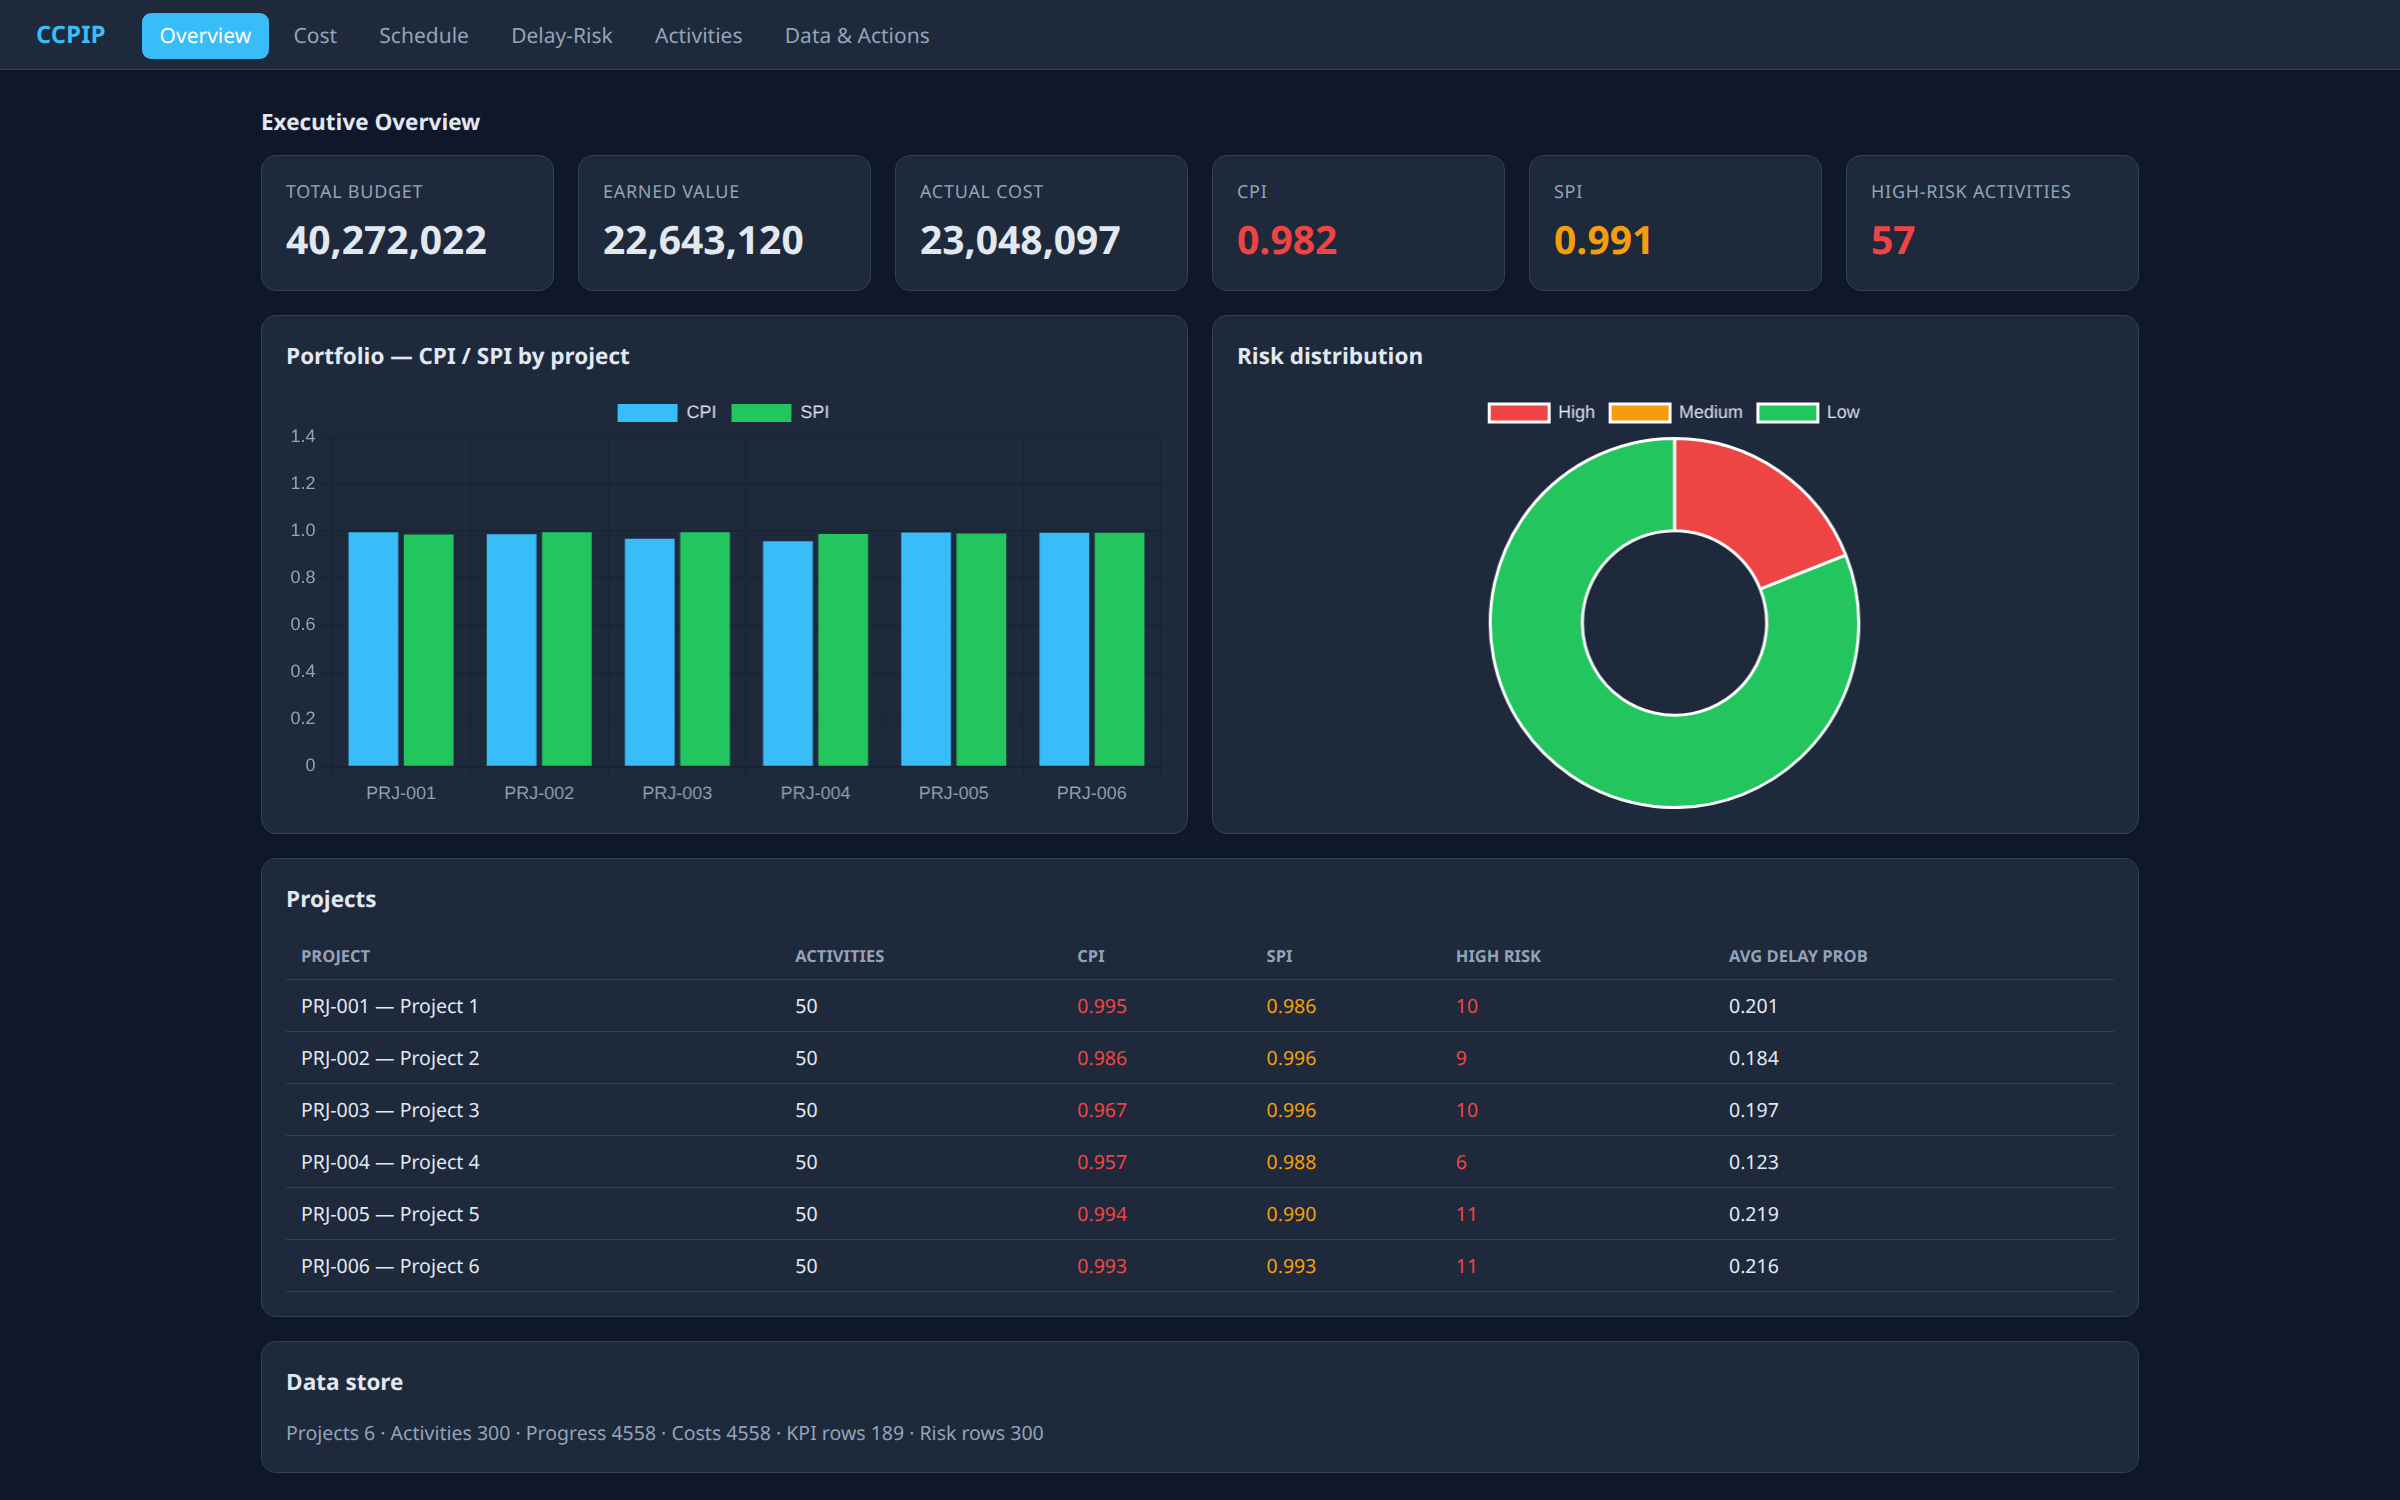
\includegraphics[width=\linewidth]{figures/fig_overview.png}\\[1pt]{\scriptsize (a) Overview}\end{minipage}\hfill
\begin{minipage}[t]{0.325\textwidth}\centering
  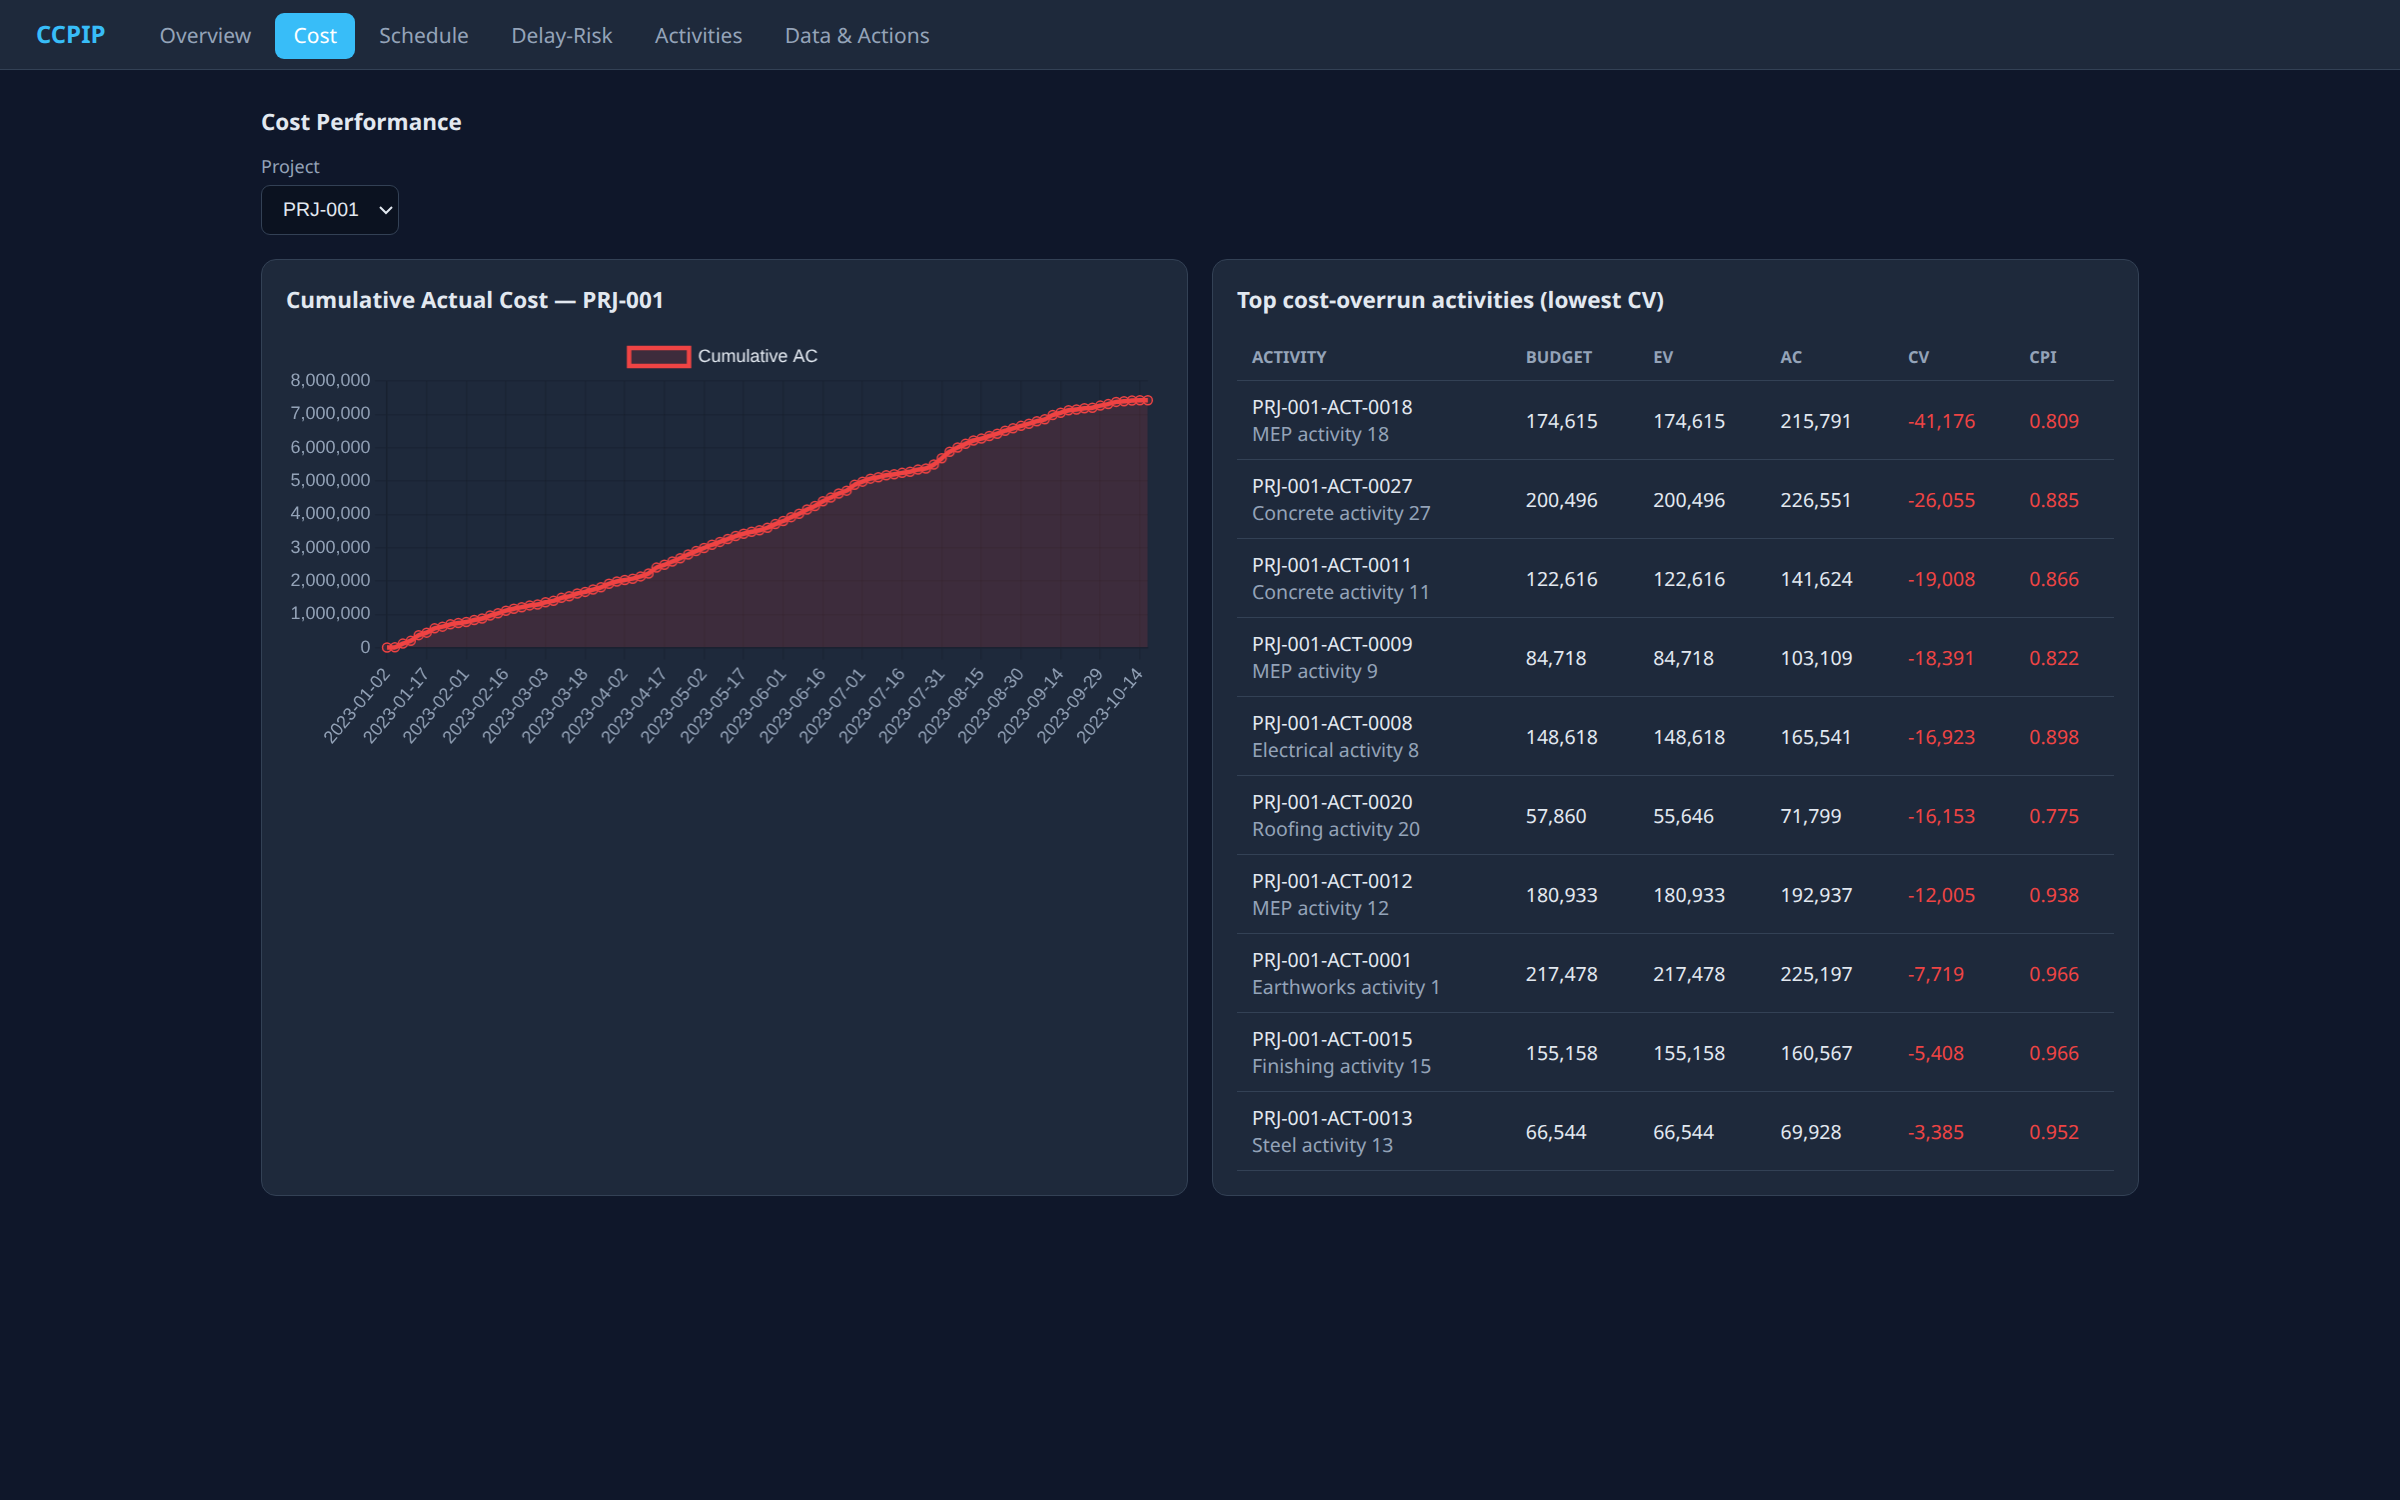
\includegraphics[width=\linewidth]{figures/fig_cost.png}\\[1pt]{\scriptsize (b) Cost}\end{minipage}\hfill
\begin{minipage}[t]{0.325\textwidth}\centering
  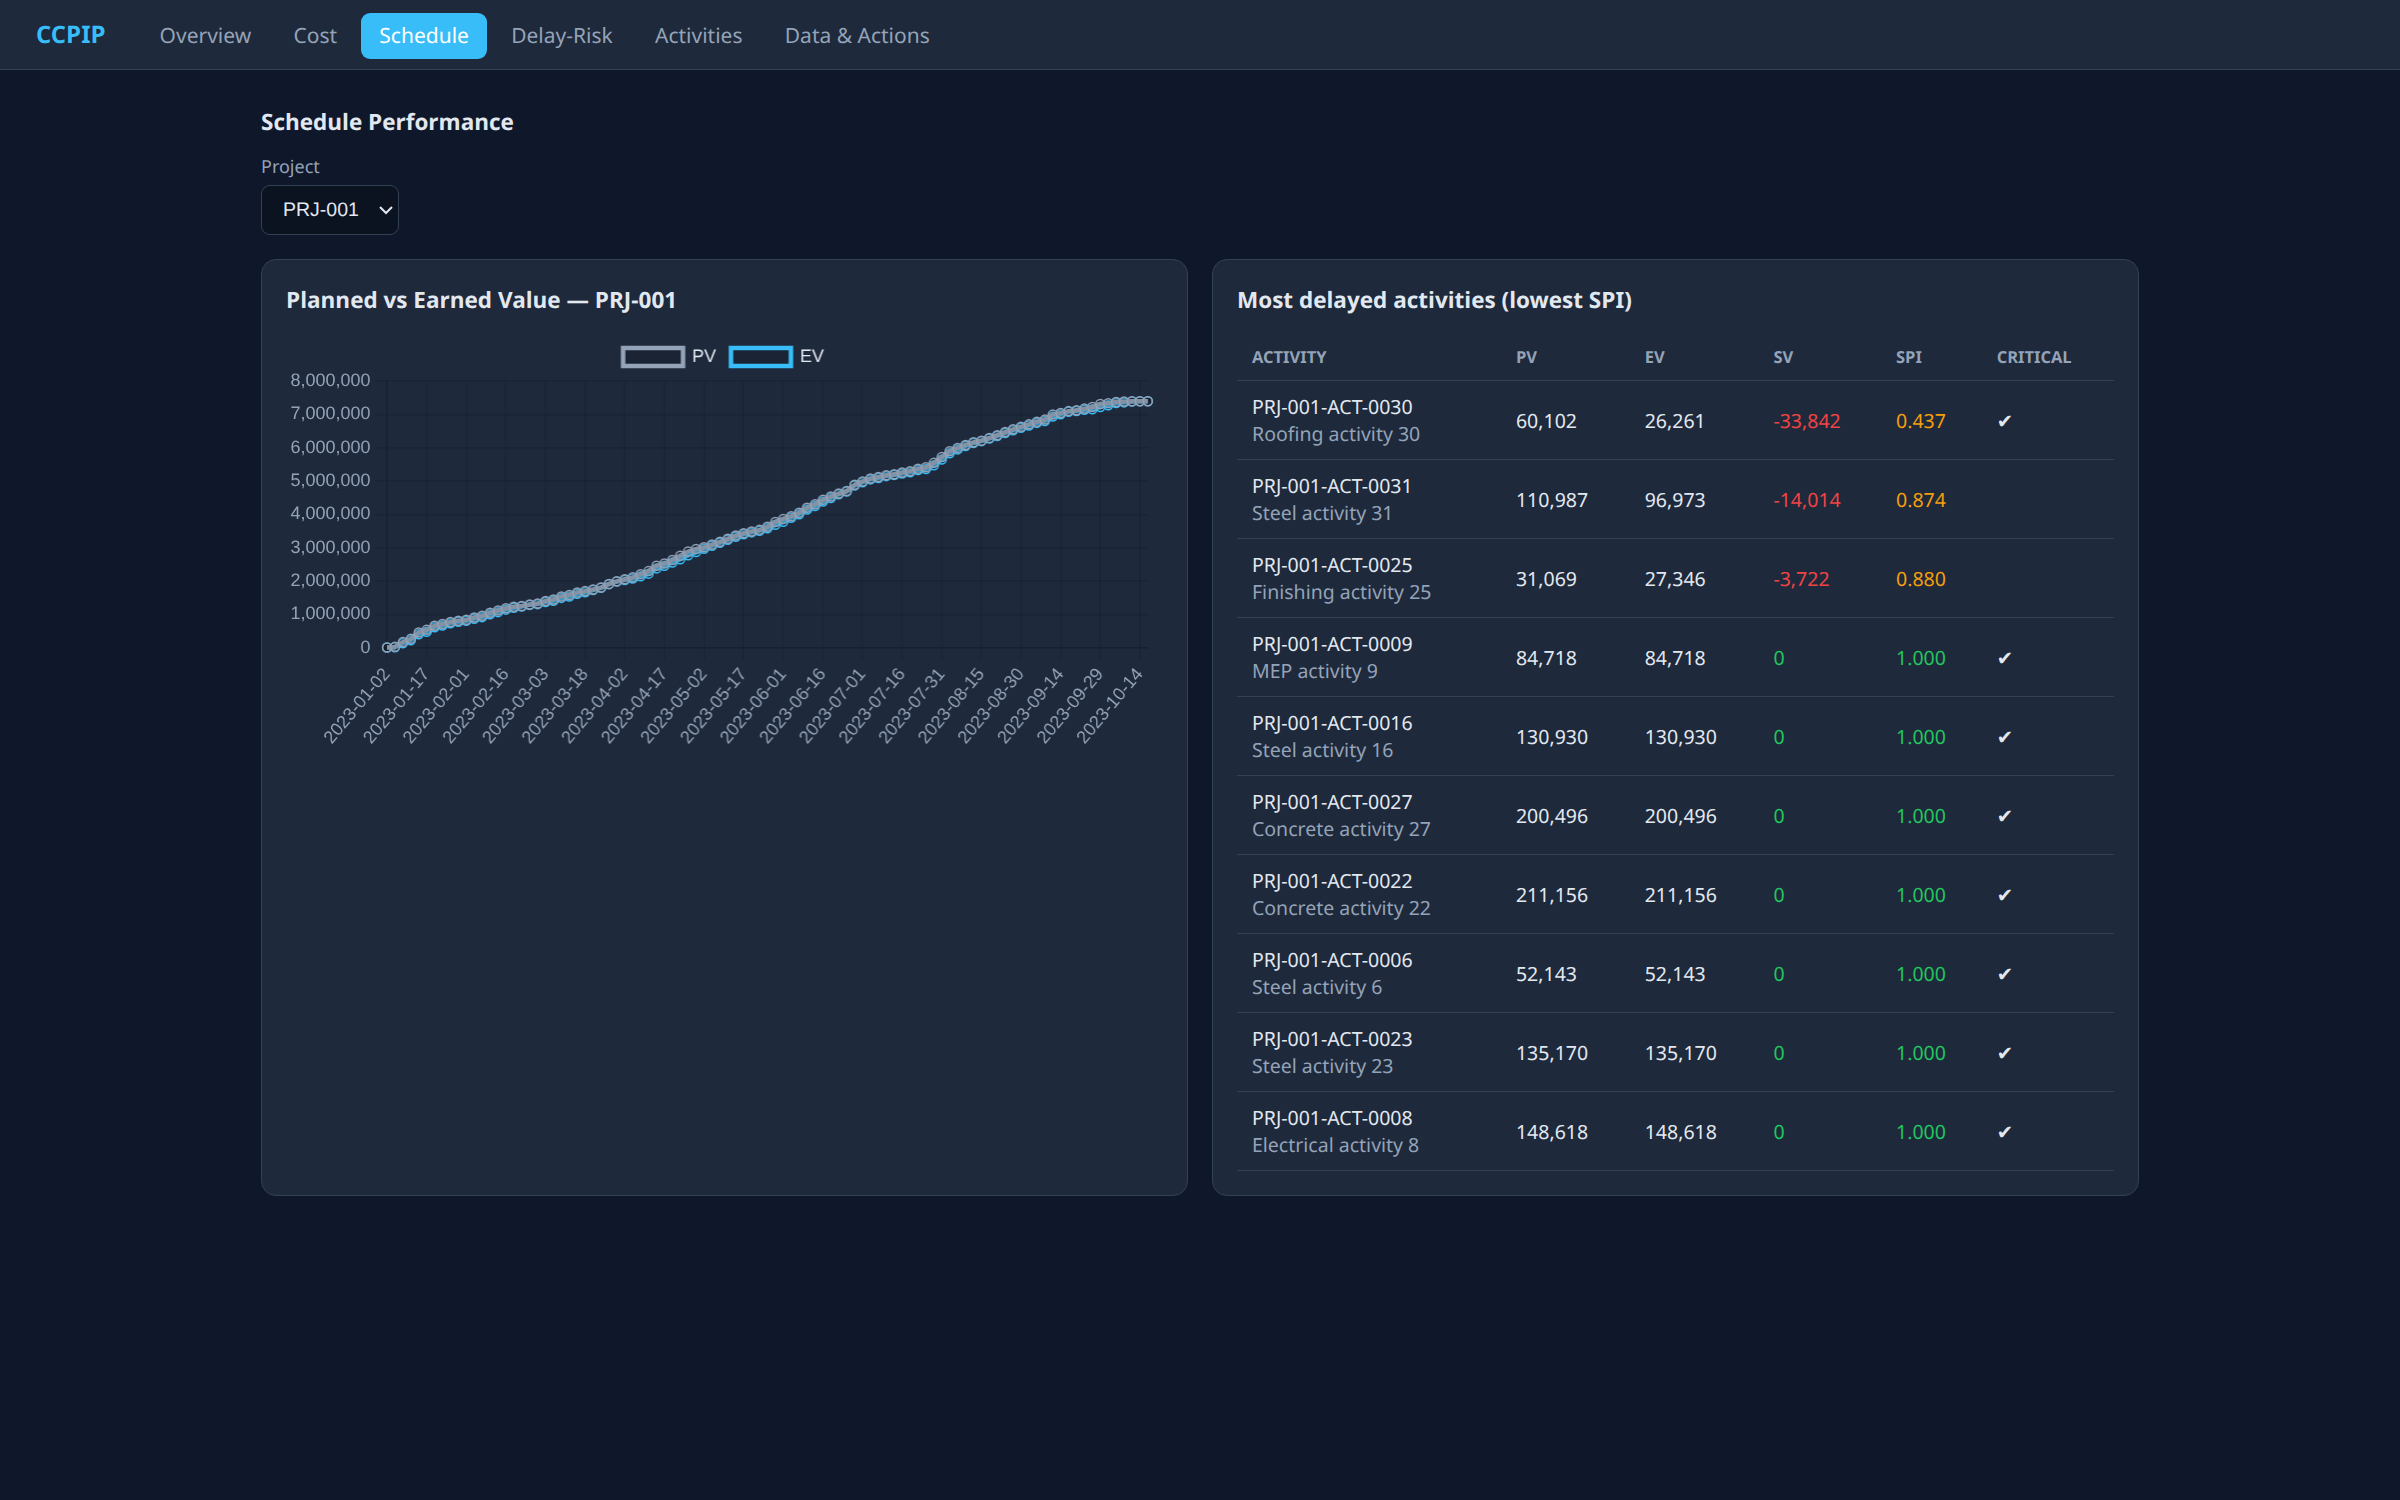
\includegraphics[width=\linewidth]{figures/fig_schedule.png}\\[1pt]{\scriptsize (c) Schedule}\end{minipage}\\[6pt]
\begin{minipage}[t]{0.325\textwidth}\centering
  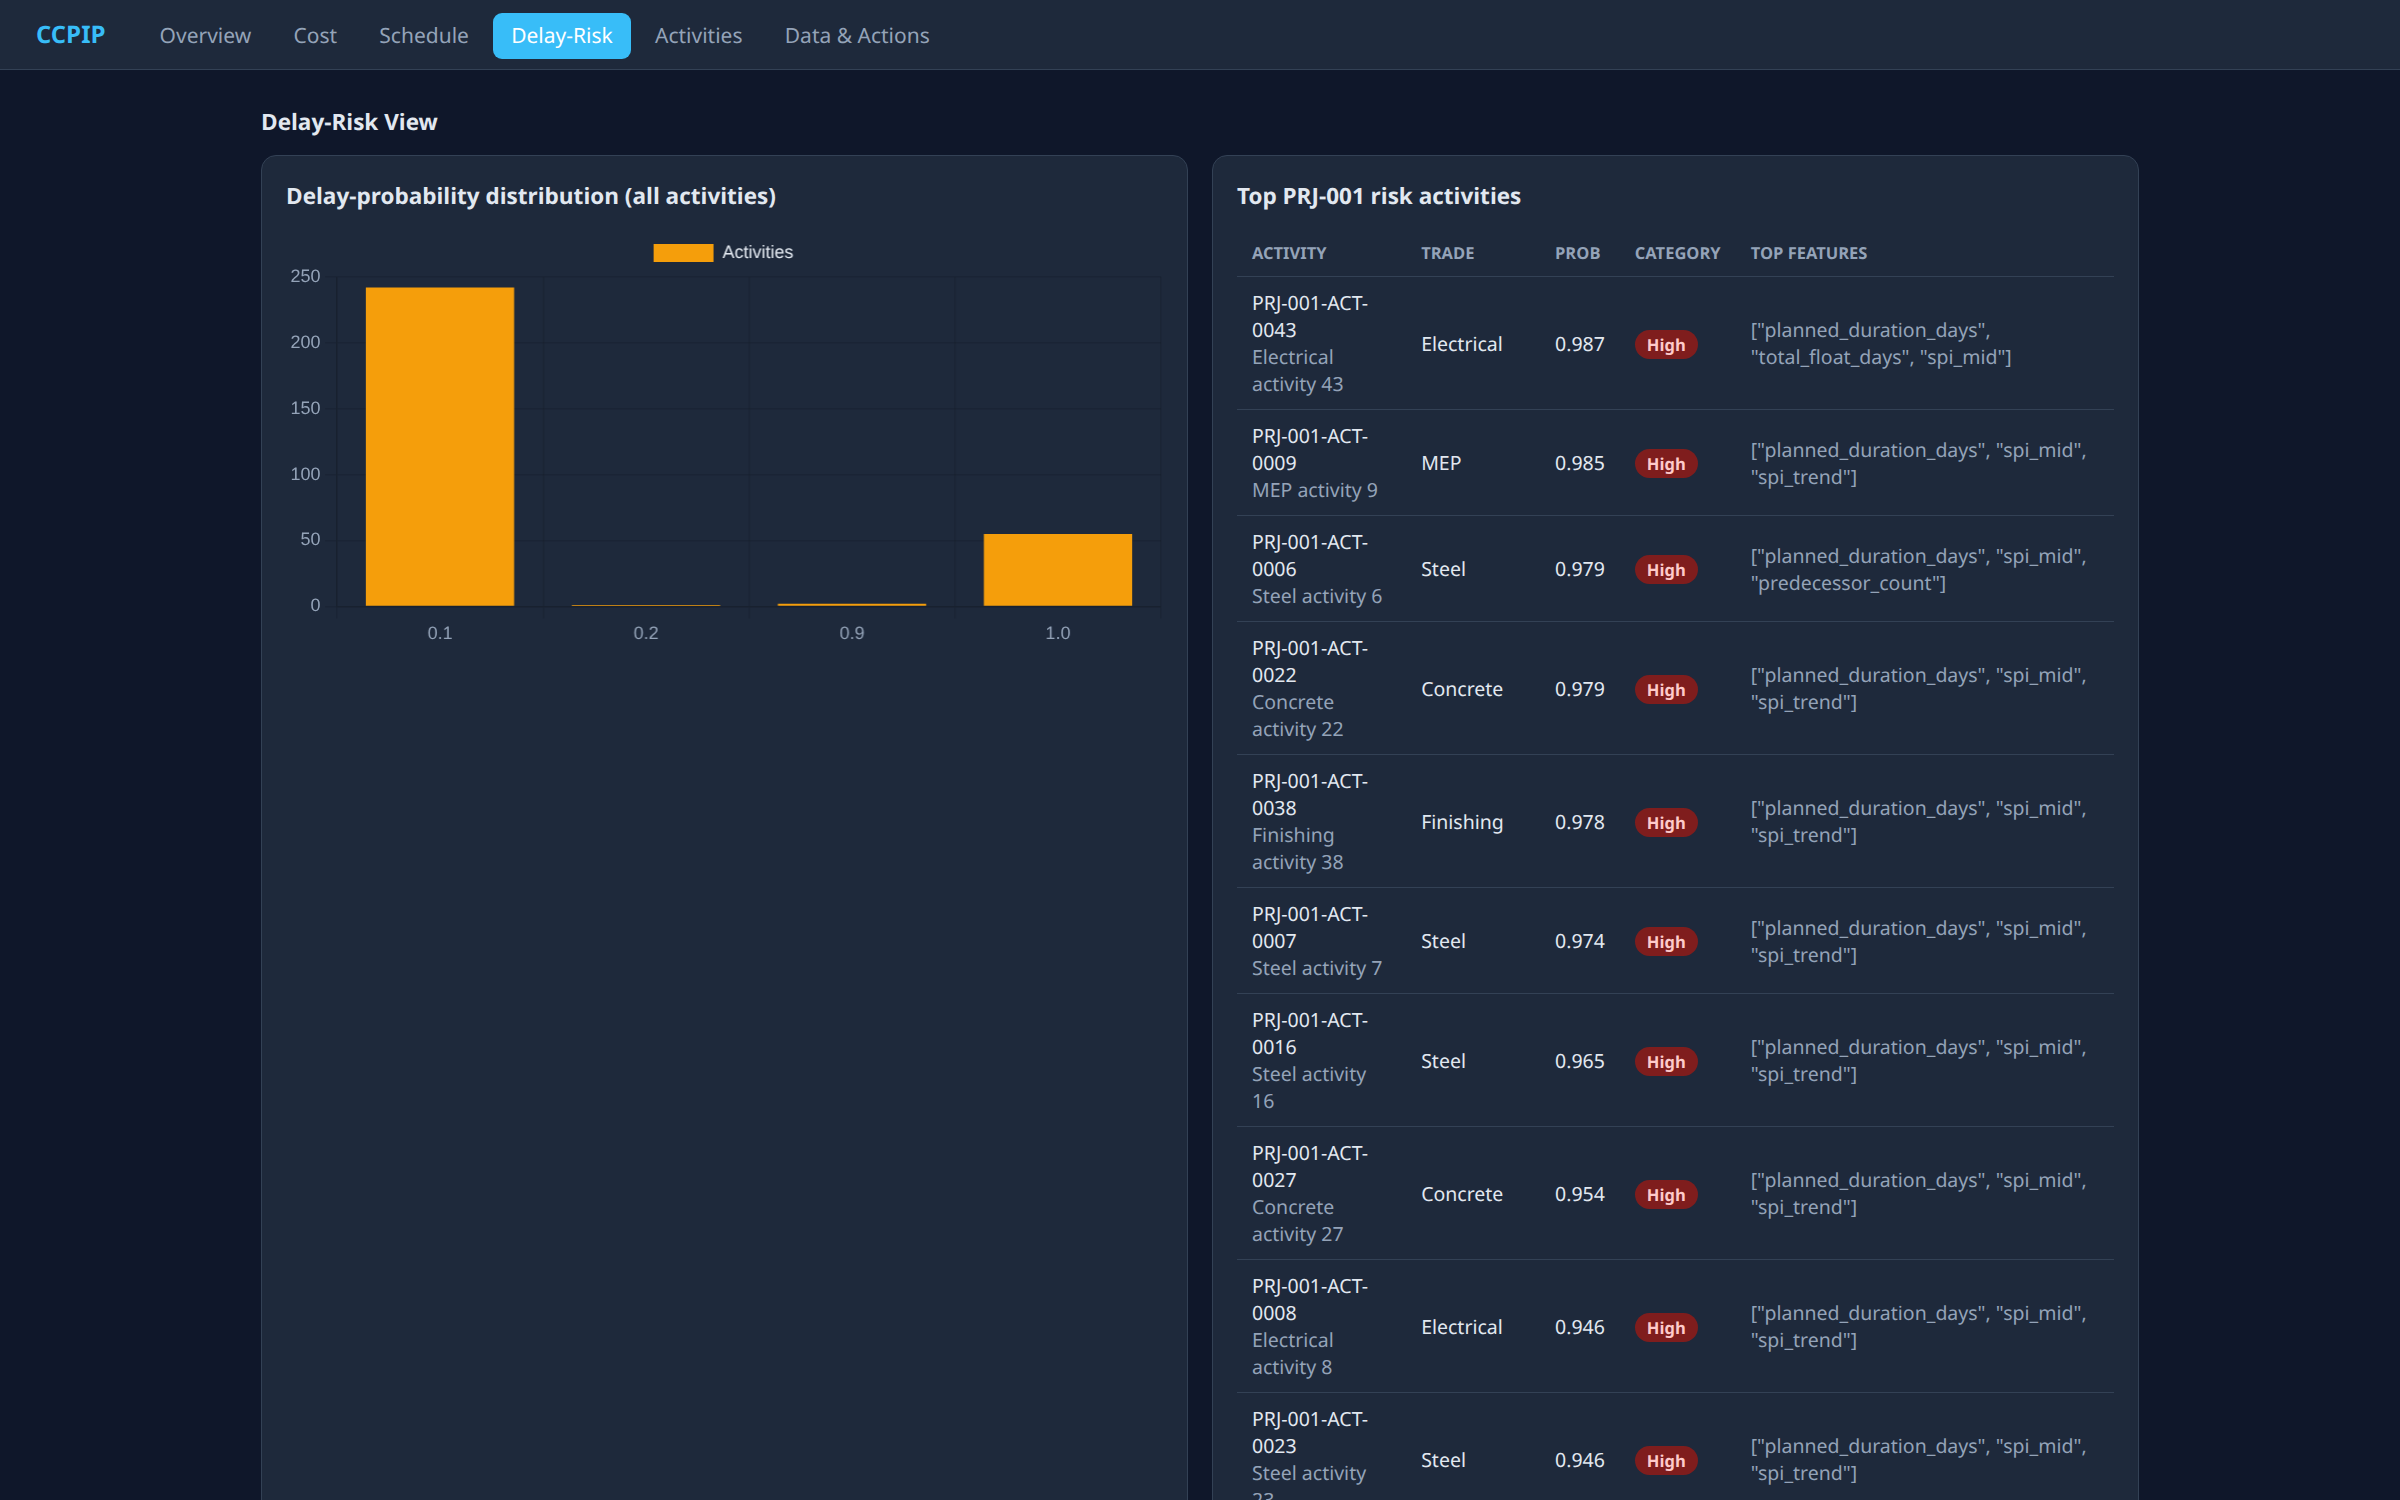
\includegraphics[width=\linewidth]{figures/fig_risk.png}\\[1pt]{\scriptsize (d) Delay risk}\end{minipage}\hfill
\begin{minipage}[t]{0.325\textwidth}\centering
  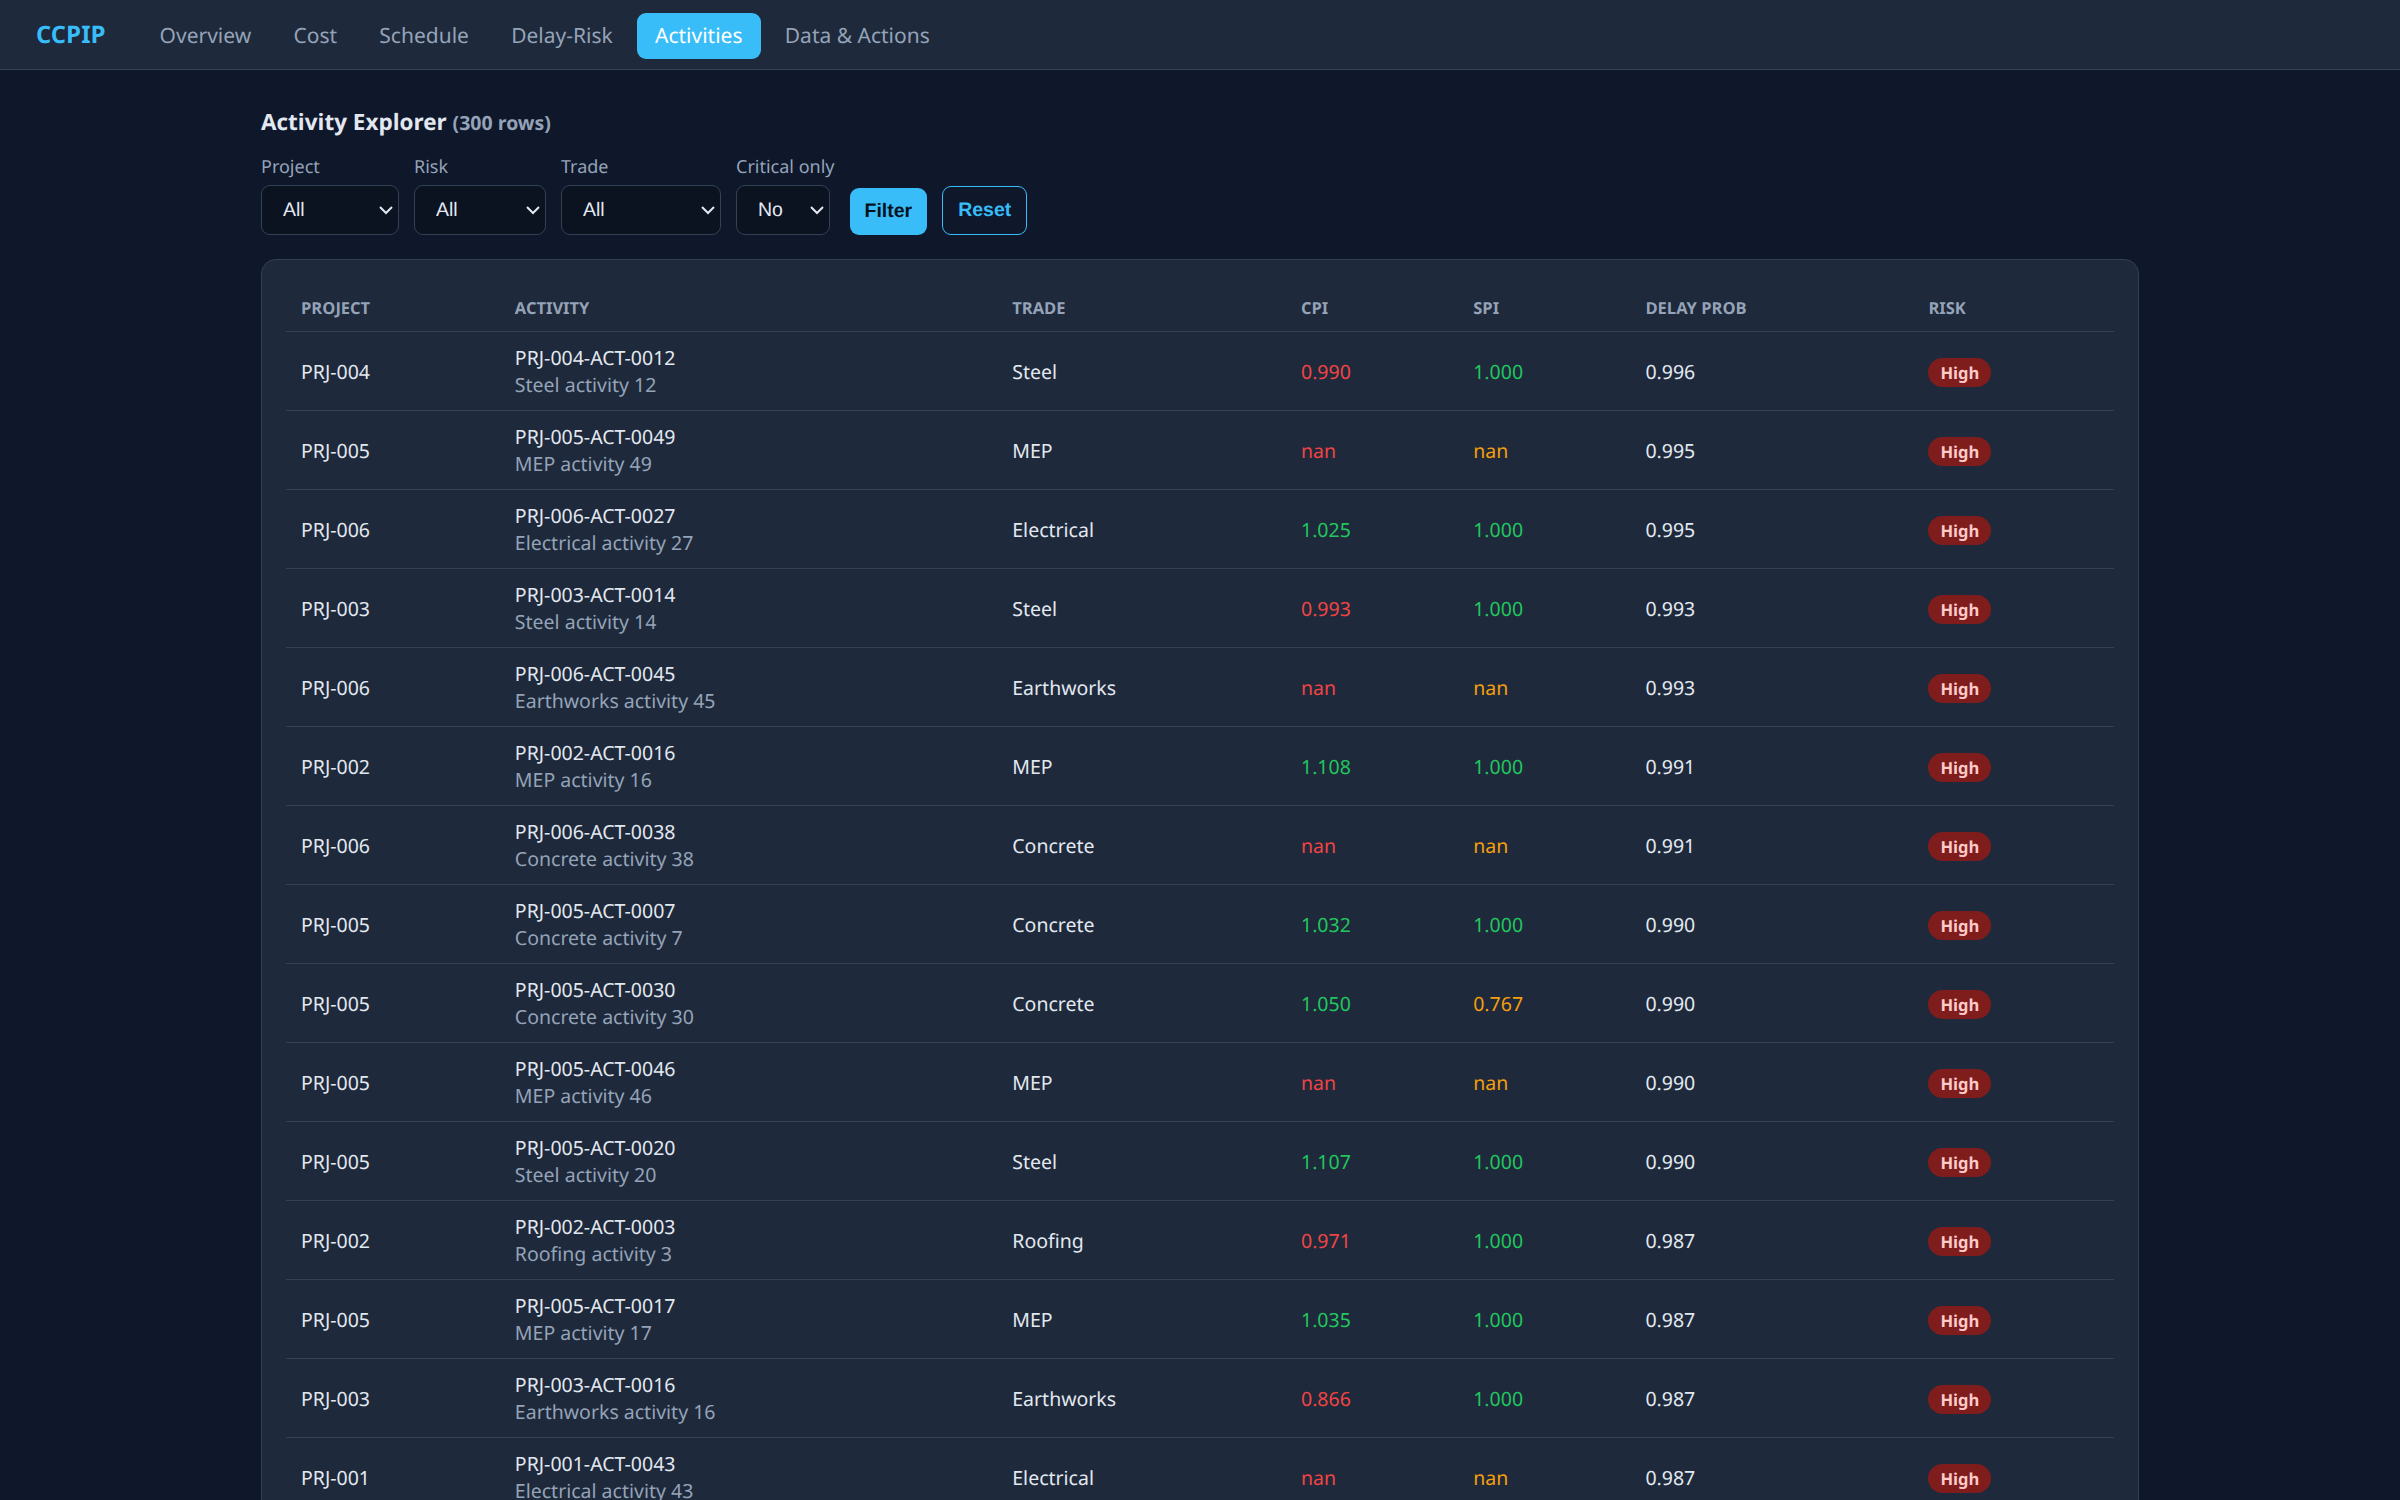
\includegraphics[width=\linewidth]{figures/fig_activities.png}\\[1pt]{\scriptsize (e) Activities}\end{minipage}\hfill
\begin{minipage}[t]{0.325\textwidth}\centering
  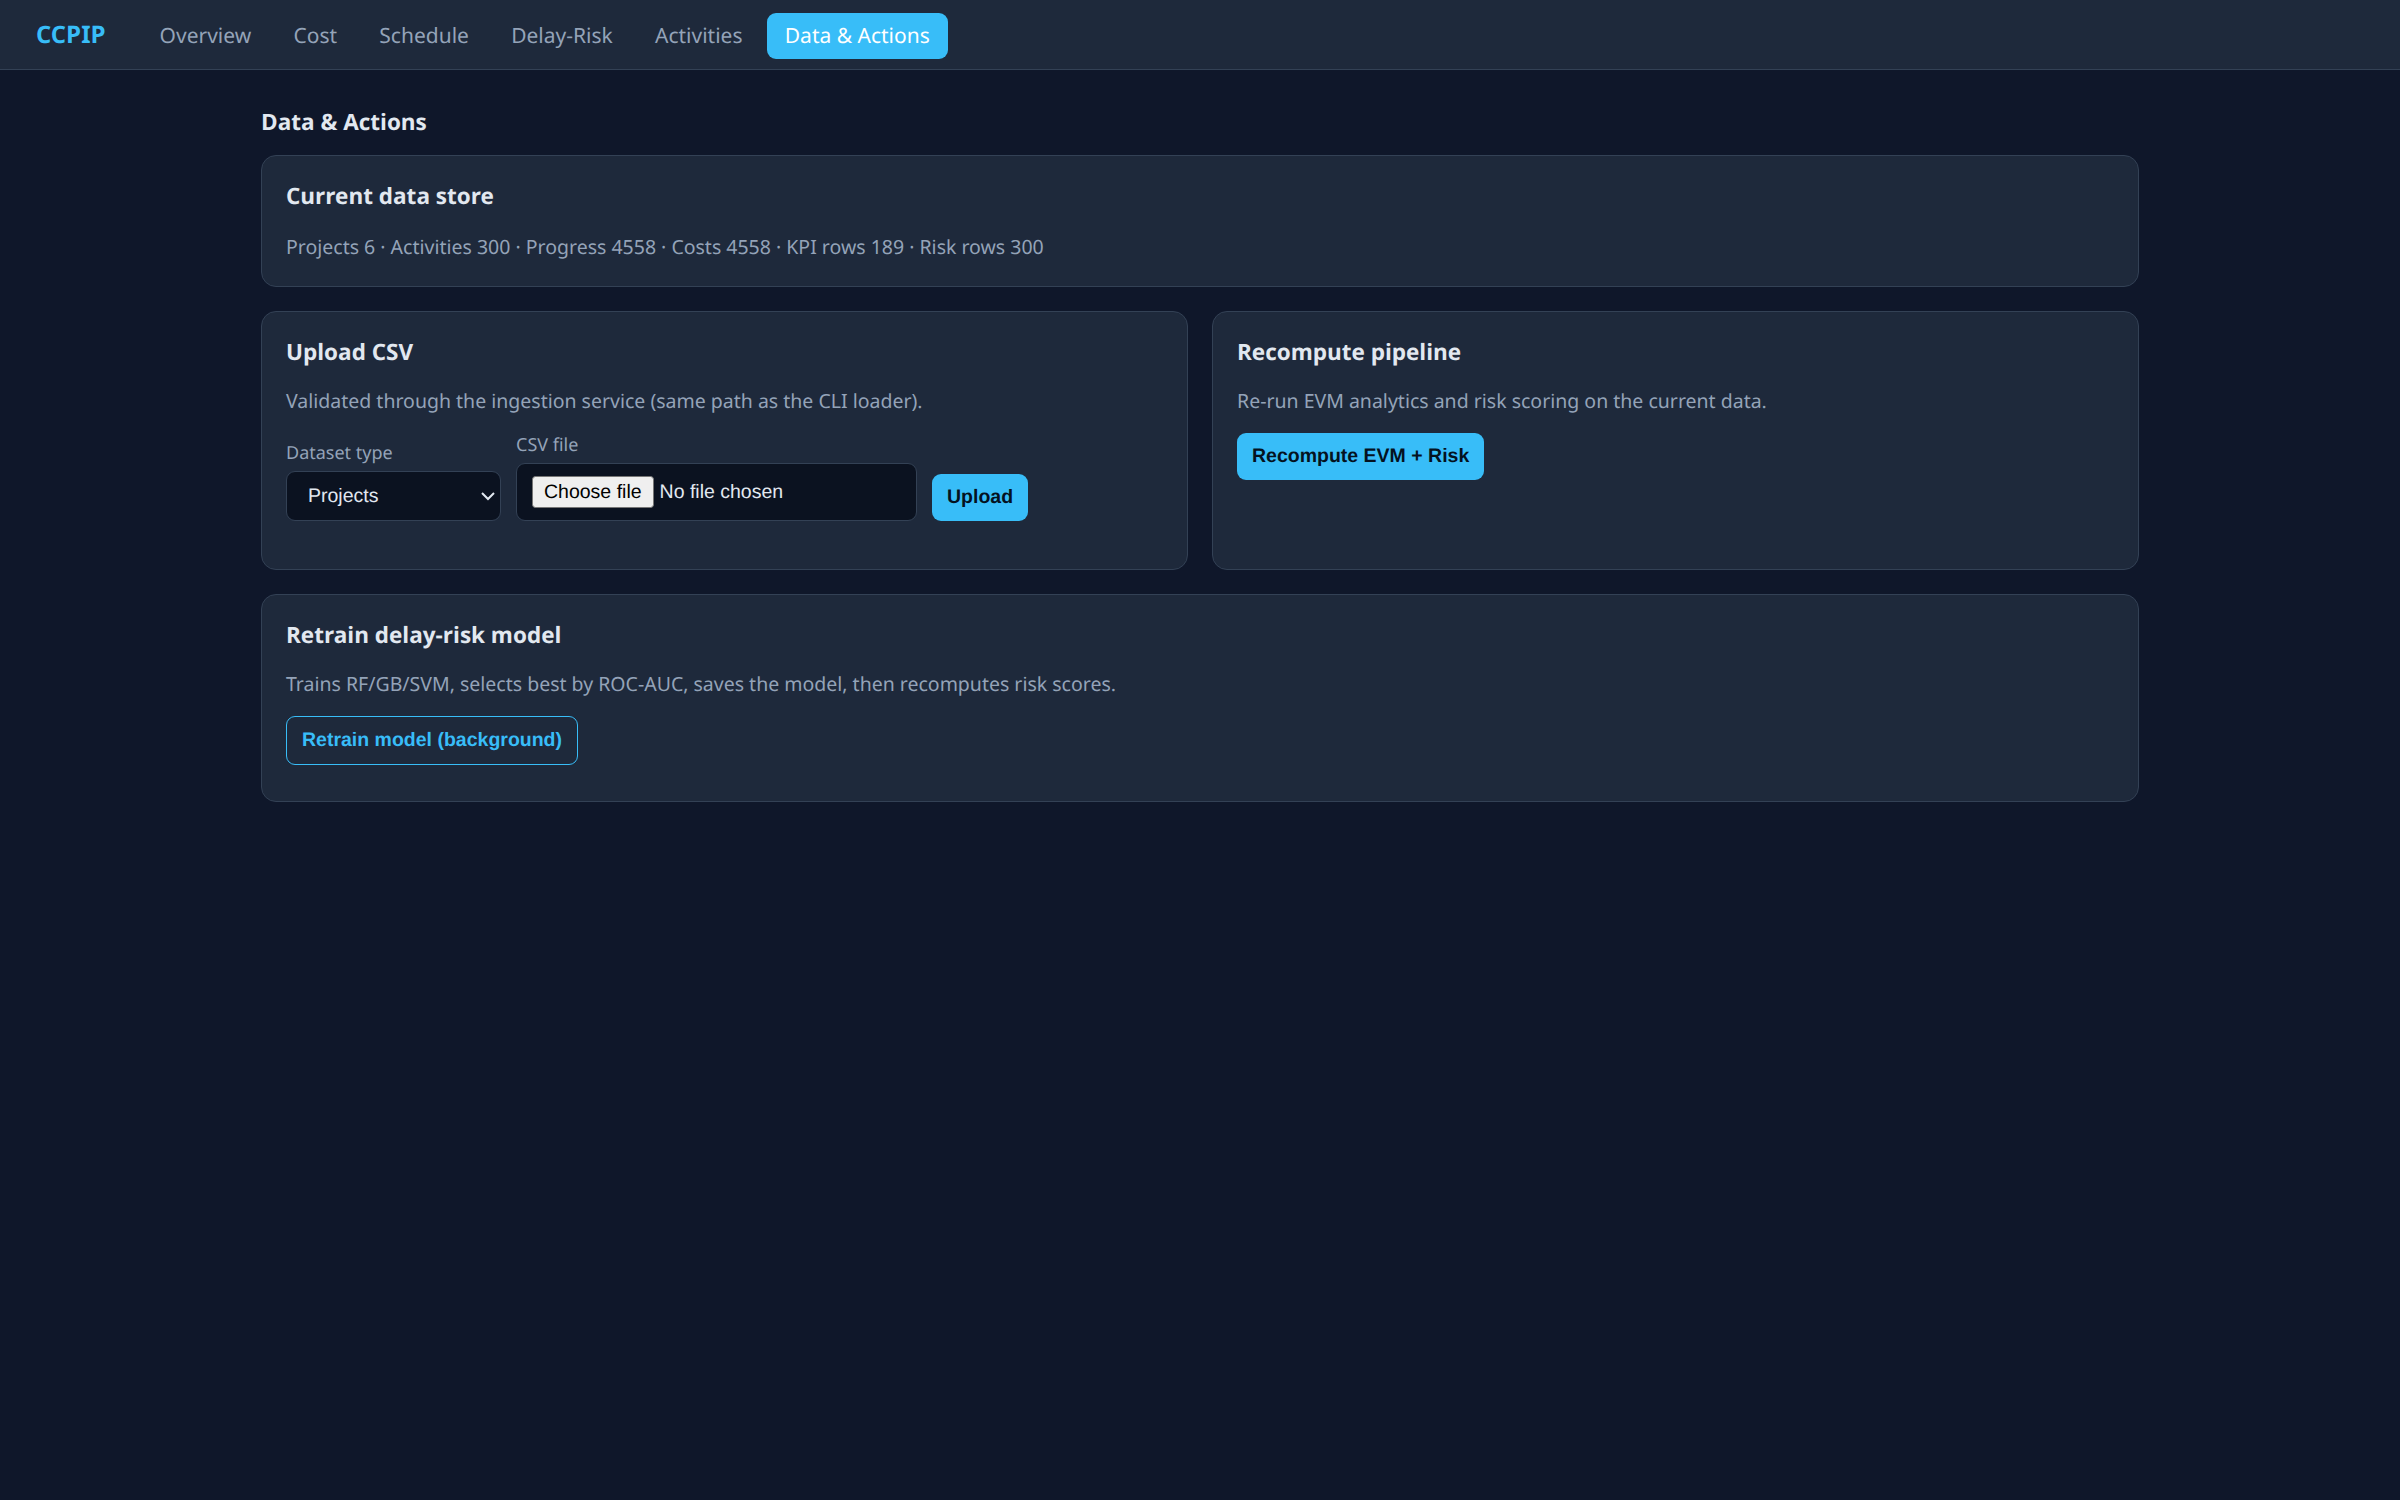
\includegraphics[width=\linewidth]{figures/fig_data.png}\\[1pt]{\scriptsize (f) Data \& actions}\end{minipage}
\caption{The six dashboard pages of the running platform: (a) executive overview with portfolio KPIs and risk distribution; (b) cumulative actual cost and cost-overrun activities; (c) planned-versus-earned S-curve with most-delayed activities; (d) delay-probability distribution and ranked high-risk activities; (e) filterable activity explorer; (f) data-and-actions console for validated upload, recomputation, and retraining.}
\label{fig:overview}
\end{figure*}

\subsection{Operational Workflow Walkthrough}

To make the evaluation concrete, consider a representative operational sequence using the platform.

\textbf{Step 1 --- data arrival.} A site engineer submits a batch of progress records through the ingestion endpoint. Each record carries an activity identifier, a timezone-aware timestamp, a percent-complete value, and earned and planned values. The service validates every field: a percent value of 150, a naive timestamp, or an unknown activity identifier is rejected with a diagnostic, while well-formed records are upserted idempotently.

\textbf{Step 2 --- analytical refresh.} The analytics worker determines each project's status date and recomputes the Earned Value indicator set for every activity at or before that date. A planner reviewing the dashboard immediately sees updated CPI, SPI, and forecasts, because the curated views resolve to the latest KPI rows.

\textbf{Step 3 --- predictive scoring.} The risk service extracts the feature vector for each activity from the same database state and scores it with the persisted model. The resulting probability is bucketed into a risk category and written alongside the most influential features, so that a planner can see not only that an activity is risky but which factors drive the assessment.

\textbf{Step 4 --- decision.} A planner filters the activity explorer to High-risk activities on the critical path, reviews the ranked list, and uses the data-and-actions console to trigger a recomputation after a data correction or a retraining after new data accrues.

\textbf{Step 5 --- resilience.} If an ingestion pod fails, Kubernetes detects the loss through the readiness probe, reschedules a replacement, and restores service without operator intervention, while persistent storage preserves the database state.

This sequence demonstrates that the platform closes the loop from raw field observation to decision support without any manual reconciliation step.

\subsection{Deployment Resilience and Reproducibility}

Cluster failover evaluations confirmed self-healing behavior: terminating an active ingestion pod resulted in automatic Kubernetes rescheduling and recreation within approximately one second, with full database integrity preserved via persistent volume claims. The Horizontal Pod Autoscaler was confirmed to target the ingestion tier between two and six replicas. Table~\ref{tab:validation} consolidates the validation outcomes across all six dimensions.

\begin{table}[t]
\caption{Validation Checklist and Outcomes}
\label{tab:validation}
\centering
\footnotesize
\begin{tabular}{@{}p{2.6cm}p{3.8cm}c@{}}
\toprule
\textbf{Dimension} & \textbf{Check} & \textbf{Result} \\
\midrule
EVM correctness & CV/SV/CPI/SPI identities & 189/189 \\
Ingestion integrity & Records ingested, zero rejects & 19,017 \\
End-to-end & Row counts, views, bounds & Passed \\
Self-healing & Pod rescheduled after deletion & $\sim$1~s \\
Autoscaling & HPA 2--6 replicas & Active \\
Reproducibility & Seeded, one-command launch & Passed \\
\bottomrule
\end{tabular}
\end{table}

\subsection{Statistical Interpretation of the Classifier Comparison}

The three classifiers exhibit complementary strengths that merit quantitative interpretation. Gradient Boosting attains the highest discrimination (ROC-AUC 0.976) with the lowest cross-validated standard deviation in ROC-AUC (0.011), indicating that its ranking quality is both high and stable across folds. Random Forest attains the highest recall (0.856) but the lowest precision (0.700), a profile that is desirable when the cost of missing a delay outweighs the cost of a false alarm, but that produces noisier alerts. The calibrated SVM attains the highest accuracy (0.920) and F1 (0.784) with a balanced precision-recall profile, making it the most defensible choice when alerts are to be triaged by human planners. Because the platform selects by ROC-AUC while retaining all three candidates for comparison, it can accommodate the differing operational preferences of cost-sensitive and schedule-sensitive stakeholders.

The gap between accuracy and ROC-AUC across models is instructive. Random Forest's accuracy of 0.900 sits below Gradient Boosting's 0.913, yet its ROC-AUC gap is larger (0.960 versus 0.976), showing that the two metrics rank the models differently. This divergence is precisely why a single-metric evaluation of delay-risk classifiers is inadvisable, and why the platform reports the full metric set.

\subsection{Sensitivity to the Delay Threshold}

The delay threshold $\tau$ in Equation~\eqref{eq:label} controls the base rate of the positive class and therefore the difficulty of the classification problem. A small $\tau$ labels nearly every activity as delayed, inflating accuracy while destroying discriminative value; a large $\tau$ labels very few activities as delayed, producing a class imbalance that penalizes recall. The chosen threshold yields a positive rate of 19\%, which is sufficiently balanced to support stratified cross-validation and sufficiently realistic to reflect that most activities finish broadly on time while a minority slip materially. Because $\tau$ is an explicit, configurable parameter of the generator, the sensitivity of the entire pipeline to this choice can be studied systematically.

\subsection{Reproducibility Contract}

Reproducibility is treated as a first-class property rather than an afterthought. The contract comprises four elements. First, a \emph{seeded generator} ensures that the dataset is a deterministic function of its configuration, so that identical configuration yields identical data. Second, a \emph{versioned schema} ensures that the structure into which data is loaded is fixed by migrations. Third, a \emph{single shared image} ensures that all services execute the same code. Fourth, a \emph{one-command launcher} ensures that the full pipeline executes without manual intervention. Together these elements satisfy the reproducibility condition of the problem statement: the mapping $\Phi$ is a function of its inputs and seed alone.

\subsection{Threats to Validity}

\textbf{Construct validity.} The delay label is defined relative to planned finish dates. If planned dates are themselves optimistic, the label measures schedule conservatism as well as real slippage. This is a property of any schedule-based label and is transparently parameterized by $\tau$.

\textbf{Internal validity.} The dataset is synthetic. Its feature-label relationships are generated by an explicit delay model, so a classifier can recover them with higher fidelity than on real data where unmodeled factors intervene. The reported ROC-AUC should therefore be read as an upper bound on what a similarly configured model might achieve on field data, not as a field-data estimate.

\textbf{External validity.} The evaluation spans six projects and 300 activities, a scale adequate to exercise every pipeline stage but smaller than an enterprise portfolio. The architectural claims (integrity, correctness, resilience, reproducibility) are scale-invariant, whereas the statistical claims (specific ROC-AUC and F1 values) are dataset-dependent and would require recalibration on real portfolios.

\textbf{Conclusion validity.} Cross-validated metrics with reported standard deviations guard against drawing conclusions from a single favorable split. The multi-metric comparison guards against single-metric overfitting. The verification protocol guards against silent numerical defects.

\subsection{Discussion}

The results substantiate the central thesis: a single reproducible platform can unify ingestion, EVM analytics, predictive risk, and visualization. Three observations merit emphasis. First, the per-project status-date design was essential to meaningful EVM; without it, schedule indicators collapsed toward unity and lost discriminating power. Second, the calibration of the SVM materially improved the interpretability of the risk categories, because uncalibrated margins do not map cleanly onto probabilities. Third, the Kubernetes failover and autoscaling evidence demonstrates that the analytical sophistication of the delay-risk model is matched by operational robustness, closing the research-to-deployment gap that motivated the work.

\subsection{Design Lessons Learned}

Several design decisions proved consequential during implementation, and documenting them is useful for practitioners building similar platforms.

\textbf{Status-date semantics are not an afterthought.} The single most impactful correction during development concerned the status date. An initial design evaluated each activity at its own final observation, which caused planned and earned values to saturate at the budget and forced the schedule index toward unity for every activity. Introducing a per-project status date---the midpoint of that project's reporting window---restored discriminating power and produced the meaningful distribution of indicators reported in Table~\ref{tab:projects}. Any platform that computes EVM must define its evaluation instant explicitly.

\textbf{Idempotency enables iterative correction.} Because ingestion upserts and the analytical workers replace their outputs per activity, the entire pipeline can be re-run after a data correction without manual cleanup. This property converts what would otherwise be a fragile, one-shot process into a robust, repeatable one, and it is a direct consequence of the three-tier separation between facts and computed outputs.

\textbf{Environment namespacing prevents silent failures.} Kubernetes injects service-discovery variables into every pod. An application setting that shares a name with an injected variable is silently overridden, producing startup failures that are difficult to diagnose. Prefixing all settings eliminated an entire class of deployment defects and is a lesson that generalizes to any containerized application deployed behind Kubernetes services.

\textbf{Calibration matters for interpretability.} Uncalibrated classifier margins are ordinal at best; they rank activities but do not yield probabilities that can be thresholded into meaningful risk categories. Wrapping the support vector machine in a calibration step produced probabilities that map sensibly onto the Low, Medium, and High categories, making the risk output actionable rather than merely directional.

\textbf{Reproducibility must be engineered, not assumed.} Reproducibility emerged not from a single technique but from the composition of a seeded generator, a versioned schema, a shared image, and a one-command launcher. Removing any one of these elements would break the reproducibility contract, which is why it is treated as an explicit design requirement (R9) rather than an incidental property.

\subsection{Practical Implications}

The platform has concrete implications for three groups of practitioners.

\textbf{For project-control engineers,} the platform replaces a manual, spreadsheet-bound reporting cycle with an automated pipeline in which validated data flows directly into verified Earned Value indicators. The status-date convention ensures that indicators reflect a coherent reporting instant, and the validation gate ensures that corrupted records are caught at the boundary rather than silently propagating into reports.

\textbf{For project managers,} the pairing of retrospective EVM with forward-looking delay-risk scores converts reporting from a post-mortem into an early-warning system. The activity explorer surfaces the specific activities that carry elevated delay probability, and the risk categories provide a triage mechanism that directs attention where intervention is most valuable. The dashboard's ability to display both aggregate project health and per-activity risk addresses the observation that healthy aggregate indicators can mask localized vulnerability.

\textbf{For the research community,} the platform demonstrates that the analytical contributions of the literature---Earned Value formulations, probabilistic reliability methods, and machine-learning classification---can be composed into a single reproducible artifact rather than remaining isolated demonstrations. The explicit reproducibility contract provides a template that other construction-informatics studies could adopt, enabling results to be regenerated from an artifact alone.

\textbf{For platform engineers,} the deployment topology illustrates how a data-intensive analytical application can be packaged for cloud-native operation with modest effort. The separation of a long-running web tier from one-shot analytical jobs, the use of health probes to gate traffic, and the namespacing of configuration to avoid collisions with injected service variables are generalizable patterns that apply well beyond construction informatics.

The broader significance of these implications is that the barrier to deploying analytical project control is primarily architectural rather than algorithmic. The individual techniques are mature; what has been missing is their composition into a system that is trustworthy, reproducible, and operationally robust. This work suggests that closing that compositional gap is both feasible and valuable.

\subsection{Comparison with Prior Reported Results}

Table~\ref{tab:benchmark} positions the platform's quantitative outcomes against values reported in the cited literature. Direct numerical comparison is necessarily approximate, because prior studies evaluate on different datasets and task definitions; nonetheless, the table situates the present results within the range of what the field reports. The delay-risk discrimination achieved here (ROC-AUC 0.976) is at the high end of the range typically reported for construction delay classifiers, which is expected given the controlled synthetic dataset and is appropriately qualified by the threats-to-validity discussion. The schedule-adherence figures are broadly consistent with the RealCONs findings, and the automated pipeline's zero-rejection ingestion corroborates the data-continuity benefits those authors attributed to structured capture. The deployment-recovery figure has no direct antecedent in the reviewed literature, because prior systems did not report container-level resilience; this is precisely the dimension that the cloud-native design adds.

\begin{table}[t]
\caption{Outcomes Relative to Representative Prior Reports}
\label{tab:benchmark}
\centering
\scriptsize
\setlength{\tabcolsep}{2.5pt}
\begin{tabular}{@{}p{2.4cm}p{1.7cm}p{2.2cm}@{}}
\toprule
\textbf{Dimension} & \textbf{This Work} & \textbf{Prior Signal} \\
\midrule
Delay-risk AUC & 0.976 & High end of ML range~\cite{sanusi2024role} \\
Schedule adherence & SPI 0.977 & SPI 1.01 vs 0.89~\cite{radman2026realcons} \\
Data continuity & 0 rejects & 7$\times$ fewer gaps~\cite{radman2026realcons} \\
Reporting latency & live recompute & 25\% reduction~\cite{gajera2023integrating} \\
Deployment recovery & $\sim$1~s & not reported \\
Visualization & web + BI & BI-centric~\cite{alsulaiti2021using} \\
\bottomrule
\end{tabular}
\end{table}

\subsection{Answers to the Research Questions}

The evaluation was framed around four research questions in Section~I; we now answer each directly.

\textbf{RQ1 (Integrity).} Yes. The ingestion service admitted 19,017 well-formed records with zero rejections while rejecting every fault-injected malformed payload with HTTP 422, demonstrating that a strict validation gate need not sacrifice throughput for correctness.

\textbf{RQ2 (Analytical correctness).} Yes. All 189 computed KPI rows satisfy the defining Earned Value identities to numerical tolerance, and the per-project status-date convention yields genuinely discriminating indicators rather than the saturated values produced by a naive evaluation instant.

\textbf{RQ3 (Predictive quality).} The candidate classifiers separate delayed from on-time activities strongly, with Gradient Boosting attaining the highest discrimination (ROC-AUC 0.976) and the calibrated SVM the best balance of precision and recall (F1 0.784). The choice of primary metric is consequential, and the platform reports the full set to support different operational preferences.

\textbf{RQ4 (Deployment resilience).} Yes. Terminating an active ingestion pod triggered automatic rescheduling within approximately one second while persistent storage preserved database integrity, and horizontal autoscaling was confirmed active across the two-to-six replica range.

Taken together, the answers indicate that the three conditions of the problem statement---enforced validation, verified indicators, and reproducible execution---hold simultaneously in a single deployable system.

\subsection{Performance and Scalability Observations}

Although the evaluation emphasized correctness and predictive quality, several operational characteristics are worth recording because they bear on practical deployment.

\textbf{Ingestion throughput.} The batch-oriented ingestion interface admitted the full 19,017-record dataset in bounded batches without error, indicating that the validation gate is not a throughput bottleneck at this scale. Because validation is stateless and the service is horizontally replicated behind a load balancer, ingestion capacity scales linearly with replica count, which is precisely the workload that the Horizontal Pod Autoscaler is configured to absorb.

\textbf{Analytical cost.} The analytics worker performs a single pass over each project's activities, fetching the status observation and computing the indicator set per activity. The cost is therefore linear in the number of activities and independent of the length of the observation history for a given status date, because only the status observation and the cumulative cost are required. This makes periodic recomputation inexpensive even as the fact tables grow.

\textbf{Scoring cost.} Delay-risk scoring extracts a fixed-length feature vector per activity and evaluates the persisted model. Inference is therefore a single matrix multiplication over the activity population and completes in well under a second for the evaluated dataset, leaving ample headroom for larger portfolios.

\textbf{Storage growth.} Because the fact tier is append-only, storage grows with the number of observations rather than being rewritten in place. This is the correct trade-off for an auditable project-control system, and it enables historical reconstruction that an in-place-update design would foreclose. Archival policies could bound long-term growth without compromising the audit trail.

\subsection{Ethical and Practical Considerations}

A platform that predicts which activities are likely to be delayed carries obligations beyond technical correctness. Predictions should inform human judgment rather than replace it: the delay-risk score is a probabilistic estimate under uncertainty, and treating it as a deterministic verdict risks misallocating attention or unfairly penalizing subcontractors whose historical delay rate contributed to the score. The platform mitigates this by surfacing the most influential features alongside each score, so that a planner can interrogate the basis of a prediction rather than accept it blindly.

Data governance is a further consideration. Project-control records frequently contain commercially sensitive cost information and personally identifiable worker data. The deployment therefore isolates credentials in a secret store, avoids embedding sensitive configuration in images, and keeps the curated reporting views separate from the operational fact tables. Production deployments would additionally require role-based access control, data-retention policies, and audit logging of who accessed which project records, all of which are identified as future work.

Finally, the synthetic dataset used in this evaluation is clearly labeled as such. Reporting results on synthetic data without qualification would be misleading; the paper states the dataset's provenance explicitly and frames the statistical results as an upper bound that requires recalibration on real portfolios.

% ============================================================================
\section{Conclusion}
% ============================================================================

This paper presented a cloud-native construction project intelligence platform that integrates project-control data across containerized microservices and automated visual analytics. By coupling Python and FastAPI ingestion pipelines, a normalized PostgreSQL relational database, automated EVM calculations, and probabilistic delay-risk scoring with interactive web and Microsoft Power BI dashboards on Kubernetes, the system addresses the historic fragmentation between field reporting, predictive analytics, and software deployment. On a reproducible activity-level dataset, the platform ingested 19,017 records with zero validation rejections, verified all Earned Value identities across 189 KPI rows, and achieved a delay-risk ROC-AUC of 0.976 with a Gradient Boosting classifier. Deployment resilience was confirmed through rapid pod self-healing and active horizontal autoscaling. The platform thereby enables project controls to operate as a proactive, data-driven operating system rather than a retrospective reporting exercise.

% ============================================================================
\section{Future Work}
% ============================================================================

Several extensions follow naturally from this work, organized below by the layer they affect.

\textbf{Data acquisition.} Incorporating live computer-vision progress feeds from on-site cameras would replace manual progress entry with automated, continuous observation, closing the remaining latency between physical execution and digital record. Complementary avenues include wearable and IoT-based resource tracking and automated extraction of progress from laser scans or photogrammetry.

\textbf{Analytical depth.} Extending the delay-risk model with schedule-network graph features---beyond the scalar feature set used here---would exploit the full topological structure of activity dependencies. Graph-neural approaches could learn representations of predecessor chains directly. The reliability formulation could be extended to propagate full distributions rather than point early-finish values, enabling confidence intervals on completion dates. A probabilistic cost-overrun model alongside delay risk would complete predictive coverage of the triple constraint.

\textbf{Validation breadth.} Validating the platform on real historical project portfolios would test generalization beyond synthetic data and motivate principled recalibration. This would also permit comparison against established industry baselines and longitudinal study of whether early warnings translate into corrective action.

\textbf{Presentation.} Embedding 4D BIM models directly within the dashboard canvas would link schedule and cost state to spatial context, allowing planners to see delay risk localized on the building model. Natural-language querying of project state would lower the barrier to insight for non-technical stakeholders.

\textbf{Operational hardening.} Adding role-based access control and multi-tenant support would prepare the platform for production deployment across multiple organizations. Offline-first synchronization with local queuing would address the connectivity constraints of remote sites. Deployment to a multi-node cloud cluster, with chaos-engineering experiments beyond single-pod failover, would strengthen the operational evidence base.

\textbf{Decision intelligence.} Closing the loop from prediction to prescription---recommending specific mitigations such as resource reallocation or schedule resequencing---would move the platform from detection toward active decision support.

% ============================================================================
\bibliographystyle{IEEEtran}
\bibliography{references}

\end{document}
